% Working report based on the supplied DA241O final term paper template.
% Overleaf main document: main.tex. Build with pdfLaTeX, Biber, then pdfLaTeX twice.
% Unfinished sections retain the template's instructional placeholders.
% The explicit page breaks before References and the back matter reproduce
% the supplied template; remove/adapt those breaks when writing the report.
\documentclass[12pt,a4paper]{article}
\usepackage[T1]{fontenc}
% Latin Modern follows the Computer Modern typography of Assignments 1 and 2.
\usepackage{lmodern}
\usepackage{microtype}
\usepackage{graphicx}
\usepackage[section]{placeins}
\usepackage{caption}
\usepackage{booktabs}
\usepackage{array}
\usepackage{amsmath}
\usepackage{csquotes}
\usepackage[backend=biber,style=apa,sorting=nyt]{biblatex}
\addbibresource{airline_references.bib}
\addbibresource{o1_stakes_appendix.bib}
\captionsetup[figure]{font=small,labelfont=bf,justification=raggedright,singlelinecheck=false,skip=7pt}
\usepackage[margin=1in]{geometry}
\usepackage{setspace}
\onehalfspacing
\setlength{\parindent}{0pt}
\setlength{\parskip}{6pt}
\usepackage{titlesec}
\titleformat{\section}{\large\bfseries}{\thesection.}{0.6em}{}
\titleformat{\subsection}{\normalsize\bfseries}{\thesubsection}{0.6em}{}
\titlespacing*{\section}{0pt}{1.2em}{0.45em}
\titlespacing*{\subsection}{0pt}{0.85em}{0.3em}
\usepackage{fancyhdr}
\pagestyle{fancy}
\fancyhf{}
\fancyhead[L]{DA241O: Managerial Economics}
\fancyhead[R]{Final Term Paper}
\fancyfoot[C]{\thepage}
\renewcommand{\headrulewidth}{0.4pt}
\setlength{\headheight}{14.5pt}
\addtolength{\headsep}{-2.5pt}
\usepackage[hidelinks]{hyperref}

% The source prints its bullets as ordinary, unindented paragraphs.
\newcommand{\templatebullet}[1]{\par\noindent\textbullet\hspace{5.88pt}#1\par}

\begin{document}
\hypersetup{pageanchor=false}
\begin{titlepage}
\centering
\vspace*{1cm}
{\Large\bfseries DA241O: MANAGERIAL ECONOMICS\par}
\vspace{0.8cm}
{\LARGE\bfseries Final Term Paper\par}
\vspace{1cm}
{\Large\bfseries From Fragmentation to Duopoly: Market Concentration and Major Consolidation Events in Indian Domestic Aviation between 2015--2026\par}
\vspace{1cm}
{\large\textbf{Team Name:} Macro Matrix\par}
{\large\textbf{Team No.:} 8\par}
\vspace{0.75cm}
{\large\textbf{Team Members:}\par}
\vspace{0.3cm}
{\large Goutham P\\
Meena Chidambaram\\
Sowmya K\\
Sweta Behera\par}
\vfill
{\large M.Tech in AI\\
Indian Institute of Science\\[0.5cm]
\textbf{Submission Date:} 20th November 2026\par}
\end{titlepage}
\hypersetup{pageanchor=true}
\setcounter{page}{1}

\section*{Abstract}
Briefly present the research problem, research question, data and methodology, main findings, and key implications.

\vspace{0.5cm}
\textbf{Keywords:} [Keyword 1]; [Keyword 2]; [Keyword 3]; [Keyword 4]

\section{Introduction}
\subsection{Background and Problem Statement}
Introduce the market, firm, sector, or policy setting being studied and explain the problem being investigated.

\subsection{Research Question}
State the primary research question.

\subsection{Research Objectives}
State the 2--3 research objectives.

\subsection{Economic Framework}
Identify the economic concept or framework used in the study and explain its relevance to the research question.

Examples may include demand and supply, market structure, information asymmetry, adverse selection, network effects, opportunity cost, principal-agent problems, or other relevant concepts from the course.

\subsection{Scope of the Study}
Specify the relevant market, geography, time period, population, firms, products, or other boundaries of the study.

\section{Literature Review}
\subsection{Existing Literature}
Review the relevant academic, government, industry, and other credible sources.

\subsection{Synthesis of Literature}
Discuss the major findings, patterns, and differences across the literature.

\subsection{Research Gap}
Clearly identify what is not adequately addressed by the existing literature and how the present study addresses this gap.

\subsection{Relevance to the Present Study}
Explain how the existing literature and identified gap inform the research question and analysis.


\subsection{O1: Ownership structure and partial stakes}
Measuring concentration at ownership-group level requires knowing who controls each airline and who holds minority stakes in rivals \parencite{obriensalop2000}. Two airlines in the sample had such cross-holdings before the Tata Group consolidated them into the Air India Group in January 2022, and their company-published stake histories are summarised below; the full schedule with sources is in Table~\ref{tab:o1-stakes} in Appendix~\ref{app:o1-stakes}.

\textbf{Vistara.} Vistara was a joint venture of Tata Sons (51\%) and Singapore Airlines (49\%) from the start of the sample \parencite{sia2015annual}, a split that Singapore Airlines restated when announcing the merger of Air India and Tata SIA Airlines in 2022 \parencite{sia2022merger}.

\textbf{AirAsia India.} AirAsia India began as a three-way venture of Tata Sons (30\%), AirAsia Investment (49\%) and Telestra (21\%) \parencite{airasia2013jv}. Tata Sons raised its stake to 41.06\% in 2015 and to 49\% in March 2016 by buying out Telestra's remaining shares \parencite{tata2016airasia}; AirAsia Berhad's reporting kept its own holding at 49\% \parencite{airasia2018q4}. Tata Sons held 51\% before the December 2020 sale in which AirAsia Investment sold 32.67\% of the company to it, leaving Tata Sons at 83.67\% and AirAsia at 16.33\% \parencite{airasia2021disposal,airasia2021results}.

Under Equation~O1.1b these minority holdings produce the partial-ownership term of MHHI: the larger the stake a rival group holds in another, the more it internalises that firm's profits, and the larger the gap between MHHI and Ownership-HHI. Once Tata Sons controls both airlines (from January 2022), the wedge is zero by construction. Because the stakes are company-reported and not directly observed in operating decisions, MHHI is treated as a measure of structure rather than of conduct.


\section{Data and Methodology}
\subsection{Research Design}
Briefly describe the research design used in the study.

\subsection{Data Sources}
Describe the data source or sources, period covered, geographic coverage, sample or number of observations where applicable, and data collection procedure where applicable.

\textbf{O1.} DGCA's Monthly Summary of Domestic Passenger Traffic, in the cleaned distribution of \textcite{kubicek2026aviationstats} (\texttt{carrier\_monthly.csv}, commit \texttt{16770ac}), gives scheduled domestic passengers by airline for January 2015--July 2026: 1,577 airline-months, 138 market-months and 26 airlines after cleaning, at national level with no fares or city pairs. Ownership stakes for the modified HHI come from company filings, with press reports for three points (Appendix~\ref{app:o1-stakes}).

\textbf{O1 data cleansing.} Nine auditable rules (Appendix~\ref{app:o1-cleaning}) coerce numeric fields, keep scheduled domestic service, sum duplicate airline-months, drop zero-passenger rows, and only flag inconsistent values, outliers and gaps; no observed value is overwritten. Shares are recomputed from passengers and sum to 100\% each month. April 2020, missing for every airline, stays empty; AirAsia India's missing 2017 is interpolated only as a sensitivity check.

\subsection{Unit of Analysis}
Clearly identify the unit of analysis, such as firm, product, transaction, household, district, city, industry, or another relevant unit.

\textbf{O1.} The unit of analysis is the market-month, for which concentration is computed. It is built from airline-months aggregated into ownership groups: Air India with Air India Express and Jet Airways with JetLite throughout, with Vistara and AirAsia India/AIX Connect joining the Air India Group from January 2022.

\subsection{Variables and Measures}
Define the key variables, indicators, measures, or categories used in the analysis.

For quantitative studies, identify the dependent variable, main explanatory variables, and relevant control variables where applicable.

\textbf{O4.} Appendix~\ref{app:o4-dictionary} defines the inputs, constructed measures, units, sample flags and source-quality conventions used in the concentration and buffer calculations.

\textbf{O1.} Appendix~\ref{app:o1-dictionary} defines the concentration indices (dependent variables), the event indicators and time trend (main explanatory variables), and the COVID and month-of-year controls.

\clearpage
\subsection{Method of Analysis}
\textbf{O4.} Descriptive index and comparative analysis assess two-group dominance and dependence on IndiGo. Each month's national passenger counts and route scheduled-flight counts are aggregated into ownership groups and ranked to calculate HHI, CR2, the leader--rival share gap and fringe share, with the leading groups identified. Route shares pool both directions of the twenty busiest airport pairs by 2025 passengers. The predefined flags are CR2 $\geq80\%$, fringe $\leq20\%$ and gap $>20$ pp, with HHI $>1{,}800$ used as a high-concentration benchmark \parencite[Section~2.1]{dojftc2023merger}. The gap and the IndiGo $\geq60\%$ frequency-share flag are study-defined; monthly exposure percentages use available pairs as their denominator, with IndiGo-only observations identified separately. Rivals' unused capacity is summed as ASK minus RPK and expressed as a percentage of IndiGo's RPK for December 2024 and December 2025. A matched December 2024--July 2026 comparison includes the top-ten subset, while H6 retains the full available April 2019--September 2026 route panel. Missing observations are excluded. Appendix~\ref{app:o4-route-preparation} records ownership conventions, source-quality checks, exclusions and worked calculations.

\textbf{O1.} Concentration indices and a segmented (interrupted time-series) regression measure how four events changed national concentration once common ownership is counted. For each market-month, brand passenger shares are $s_{it}=100\,q_{it}/\sum_j q_{jt}$, with $q$ passengers carried, and brands are summed into controlling groups $S_{gt}$ under the ownership convention above. The Herfindahl--Hirschman Index (HHI) is the sum of squared shares, from 0 to 10,000, with values above 1,800 highly concentrated \parencite{dojftc2023merger}. The modified HHI (MHHI) adds rivals' partial cross-holdings \parencite{obriensalop2000}:
\begin{align}
\text{Brand-HHI}_t &= \sum_i s_{it}^2, \qquad \text{Ownership-HHI}_t = \sum_g S_{gt}^2 \tag{O1.1a}\\
\text{MHHI}_t &= \text{Ownership-HHI}_t+\sum_{j}\sum_{k\neq j}\lambda_{jk}S_{jt}S_{kt},\qquad
\lambda_{jk}=\frac{\sum_i \gamma_{ij}\beta_{ik}}{\sum_i \gamma_{ij}\beta_{ij}} \tag{O1.1b}
\end{align}
where $\beta_{ik}$ is owner $i$'s financial stake in firm $k$ and $\gamma_{ik}$ its control share ($\gamma=\beta$ in the baseline; the alternative gives a majority owner full control). $\mathrm{CR2}=S_{(1)}+S_{(2)}$ is the two largest groups' combined share; it ignores the split below the top two, so it is reported with HHI \parencite{gandhi2026marketstructure}. Ownership-HHI $-$ Brand-HHI is the Grouping Effect and MHHI $-$ Ownership-HHI the Partial-Ownership Effect, zero from January 2022 by construction. A rise in all HHI variants is a share shift; in Ownership-HHI and MHHI only, a change of control; in Brand-HHI only, a change in reporting.

Drift points are months whose change has a modified $z$-score above 3.5 \parencite{iglewicz1993outliers}, or trend breaks from piecewise-linear fits with minimum segments of 12 months, found by dynamic programming \parencite{baiperron2003} and chosen by the Bayesian information criterion. Each index is then regressed over the 138 months:
\begin{equation}
\text{Index}_t = \alpha + \beta t + \sum_{k=1}^{4}\gamma_k\,\text{Post}_{kt} + \delta\,\text{COVID}_t + \sum_{m=2}^{12}\mu_m M_{mt} + \varepsilon_t \tag{O1.2}
\end{equation}
with $\text{Post}_{kt}$ switching on at the Jet Airways exit (May 2019), Tata acquisition of Air India (January 2022), Go First exit (June 2023) and legal mergers (December 2024), COVID covering March 2020--December 2021, and Newey--West errors with 12 lags \parencite{neweywest1987}. The $\gamma_k$ are descriptive level shifts, not causal effects. Robustness checks are in Appendix~\ref{app:o1-robust}.

\subsection{Hypotheses or Expected Relationships}
\textbf{H5 (O4): National concentration.} We expect IndiGo and the Air India Group to remain the two largest groups in every month from December 2024 to July 2026, with CR2 $\geq80\%$ and a share gap above 20 percentage points. HHI $>1{,}800$ is not tested separately, since CR2 $\geq80\%$ already implies HHI $\geq3{,}200$.

\textbf{H6 (O4): Route concentration.} We expect ownership-adjusted scheduled-flight-frequency HHI to exceed 1,800 in more than half of the available route-month observations for the selected twenty airport pairs.

\textbf{H7 (O4): Capacity buffer.} We expect rivals' unused capacity relative to IndiGo's passenger-kilometres to be lower in December 2025 than in December 2024.

\textbf{H1 (O1): Lasting event steps.} We expect each exit, acquisition and merger to produce a positive and lasting step in Ownership-HHI ($\gamma_k>0$ and significant in Equation~O1.2), so that concentration does not return to its pre-event level.

\textbf{H2 (O1): Partial-ownership wedge.} We expect MHHI to exceed Ownership-HHI before January 2022, reflecting Tata's stakes in Vistara and AirAsia India, and the difference to vanish once both join the Air India Group.

% Keep the first O4 description and figure together in this working draft.
\clearpage
\section{Descriptive and Exploratory Analysis}
\subsection{O4: National concentration trends}
Across 138 observed months (January 2015--July 2026), the top two groups' combined passenger share (CR2) rises from 60.7\% to 91.3\%, and their gap from 12.5 to 43.4 percentage points (Figure~\ref{fig:o4-national-eda}). IndiGo is first throughout; Table~\ref{tab:o4-leading-pairs} names the second group by period. Appendix~\ref{app:o4-national-summary} (Table~\ref{tab:o4-national-summary}) provides summary statistics.

The January 2022 movement partly reflects regrouping Vistara and AirAsia India/AIX Connect with the Air India Group, rather than changes in passenger volumes alone.

\begin{minipage}{\linewidth}
\captionsetup{font=small,labelfont=bf,justification=raggedright,singlelinecheck=false,hypcap=false}
\captionof{table}{Second-largest ownership group by observed period.}
\label{tab:o4-leading-pairs}
\centering
{\small\setstretch{1.0}
\begin{tabular}{@{}llr@{}}
\toprule
Period & Second-largest group & Observed months \\
\midrule
Jan 2015--Jan 2019 & Jet Airways Group & 49 \\
Feb 2019--Apr 2021 & SpiceJet & 26 \\
May--Aug 2021 & Air India Group & 4 \\
Sep 2021 & Vistara & 1 \\
Oct--Dec 2021 & Go First & 3 \\
Jan 2022--Jul 2026 & Air India Group & 55 \\
\bottomrule
\end{tabular}\par}
\vspace{3pt}
{\footnotesize\setstretch{1.1}\raggedright\textit{Note:} April 2020 is missing. Source: same passenger series as Figure~\ref{fig:o4-national-eda}.\par}
\end{minipage}

\begin{figure}[htbp]
\centering
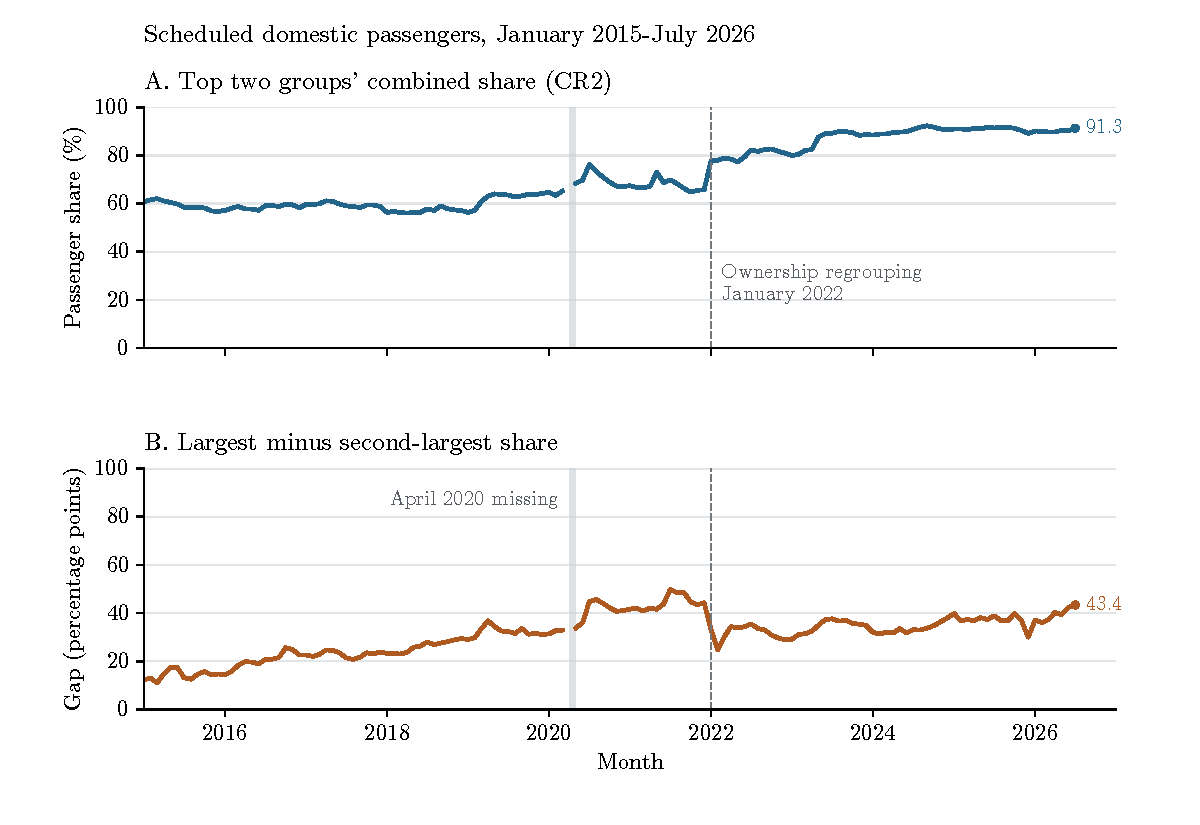
\includegraphics[width=\linewidth]{figures/o4_national_cr2_share_gap.pdf}
\caption{National concentration and share asymmetry, 2015--2026.}
\label{fig:o4-national-eda}
\vspace{2pt}
\begin{minipage}{\linewidth}
\footnotesize\setstretch{1.1}
\textit{Source:} DGCA monthly traffic via \href{https://github.com/mkubicek/india-aviation-stats/tree/16770ac59dae61ce7b80fd8bd67dd7f4cef280a6}{Kubicek (2026)}; authors' calculations.
\end{minipage}
\end{figure}

\clearpage
\subsection{O4: Route coverage and concentration}
The sample fixes the 20 busiest airport pairs by 2025 passengers, combining directions. One observation is one airport pair in one calendar month: Delhi--Mumbai in June and July count as two separate observations. There are 1,150 observations across 66 months between April 2019 and September 2026.

Panel~A of Figure~\ref{fig:o4-route-eda} counts pairs with usable data each month (12--20 in observed months). Gaps mean no retained observations, rather than zero flights.

Panel~B groups the 1,150 observations into HHI intervals of 500 points. Its horizontal axis shows HHI; its vertical axis counts observations. For example, 278 observations have HHI from 3,500 up to 4,000, so that bar has height 278. The bar heights sum to 1,150. This shows how often different concentration levels occur across the observed pairs and months, rather than how HHI changes over time.

Each observation has equal weight. Median HHI is 3,711; the middle half lies between 3,180 and 4,244. HHI uses ownership groups' approved scheduled-flight shares, not passenger shares. Appendix~\ref{app:o4-route-preparation} records preparation and exclusions.

\begin{figure}[htbp]
\centering
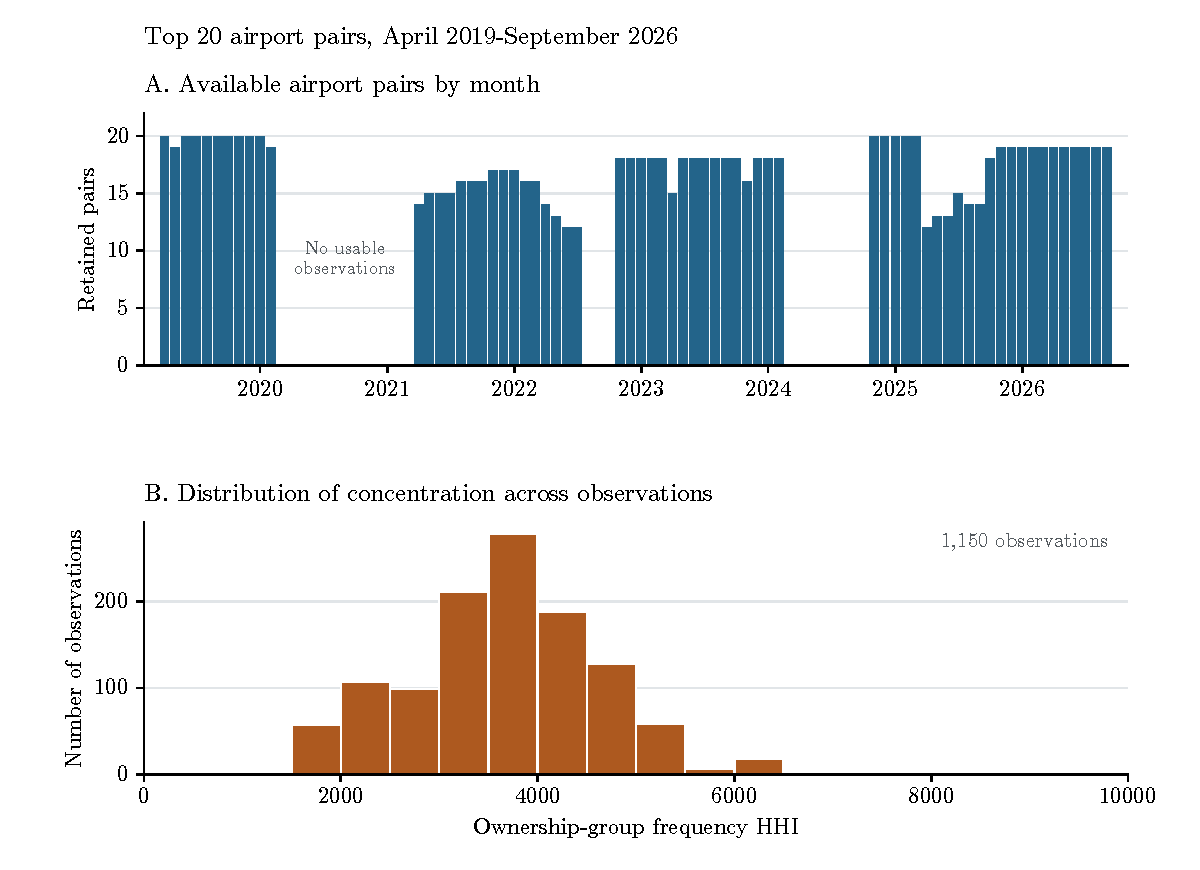
\includegraphics[width=\linewidth]{figures/o4_route_coverage_hhi.pdf}
\caption{Route-data coverage and the distribution of ownership-group frequency HHI.}
\label{fig:o4-route-eda}
\vspace{2pt}
\begin{minipage}{\linewidth}
\footnotesize\setstretch{1.1}
\textit{Source:} DGCA approved domestic schedules; authors' calculations.
\end{minipage}
\end{figure}

\clearpage
Figure~\ref{fig:o4-route-heatmap} complements the pooled histogram in Figure~\ref{fig:o4-route-eda} using the same 1,150 observations. Each row is one airport pair, ordered by 2025 passenger totals, and each column is a calendar month. Colour shows ownership-group frequency HHI on a common 0--10,000 scale; grey means no usable observation. Reading across a row shows changes for that pair, while reading down a column compares pairs in the same month. Gaps are not interpolated.

For example, Mumbai--Delhi's HHI rises from 2,071 in April 2019 to 4,146 in September 2026. The heatmap preserves this time and pair information, while the histogram shows how frequently each concentration range occurs across all observations.

\begin{figure}[htbp]
\centering
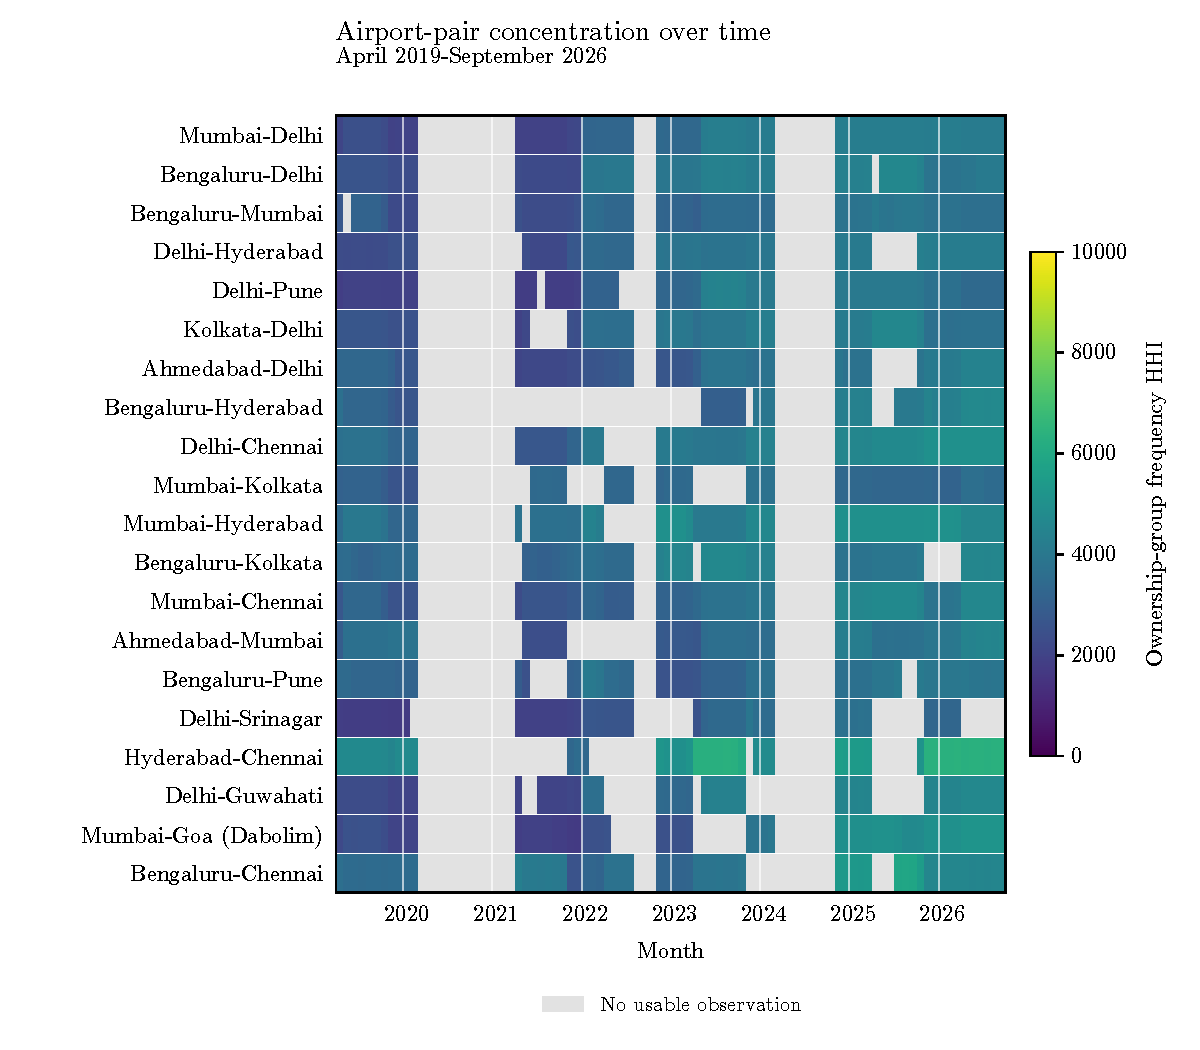
\includegraphics[width=\linewidth]{figures/o4_route_hhi_heatmap.pdf}
\caption{Ownership-group frequency HHI by airport pair and month.}
\label{fig:o4-route-heatmap}
\vspace{2pt}
\begin{minipage}{\linewidth}
\footnotesize\setstretch{1.1}
\textit{Source:} DGCA approved domestic schedules; authors' calculations.
\end{minipage}
\end{figure}

\clearpage
\subsection{O4: Capacity and passenger-traffic inputs}
Table~\ref{tab:o4-capacity-inputs} presents December 2024 and December 2025 data for scheduled domestic passenger airlines. Offered capacity, measured in available seat-kilometres (ASK), is seats offered multiplied by distance. Passenger traffic, measured in revenue passenger-kilometres (RPK), is paying passengers carried multiplied by distance. Both are reported in billions, with all airlines other than IndiGo pooled together.

IndiGo's offered capacity and passenger traffic are lower in December 2025, while both are higher for the other airlines combined. The gap between capacity and traffic supplies the input for the unused-capacity calculation in the main analysis. These national totals do not identify spare seats on a particular route or day.

\begin{minipage}{\linewidth}
\captionsetup{font=small,labelfont=bf,justification=raggedright,singlelinecheck=false,hypcap=false}
\captionof{table}{Capacity and passenger-traffic inputs for the December comparison.}
\label{tab:o4-capacity-inputs}
\centering
{\small\setstretch{1.1}\begin{tabular}{@{}llrr@{}}
\toprule
Month & Airlines & \shortstack[r]{Offered capacity\\(billion seat-km)} & \shortstack[r]{Passenger traffic\\(billion passenger-km)} \\
\midrule
Dec 2024 & IndiGo & 10.053 & 9.113 \\
Dec 2024 & Other airlines & 6.385 & 5.493 \\
Dec 2025 & IndiGo & 9.312 & 8.208 \\
Dec 2025 & Other airlines & 6.619 & 5.947 \\
\bottomrule
\end{tabular}
\par}
\vspace{4pt}
{\footnotesize\setstretch{1.1}\raggedright\textit{Source:} DGCA monthly airline traffic via \href{https://github.com/mkubicek/india-aviation-stats/tree/16770ac59dae61ce7b80fd8bd67dd7f4cef280a6}{Kubicek (2026)}; authors' calculations.\par}
\end{minipage}

\clearpage
\subsection{O1: Concentration trends and data quality}
The raw file has no missing fields, duplicates or impossible load factors; the noise is in coverage and small carriers. Dropping the 23 unexplained, immaterial outlier flags moves Brand-HHI by at most 70.6 points and Ownership-HHI and MHHI by at most 34.5. AirAsia India has no 2017 rows, so the headline series, overstated by about 165--171 points in those months, stays as published. Brand- and Ownership-HHI average 3,249 and 3,447 and never fall below the 1,800 line \parencite{dojftc2023merger}. Table~\ref{tab:o1-periods} shows every measure rising across the four periods while the fringe outside the top two groups shrinks from 41.3\% to 9.3\%. IndiGo's share is 2.81 times the second group's in July 2026. Appendix~\ref{app:o1-tables} gives summary statistics.

\begin{minipage}{\linewidth}
\captionsetup{font=small,labelfont=bf,justification=raggedright,singlelinecheck=false,hypcap=false}
\captionof{table}{O1: Concentration measures by period (period means).}
\label{tab:o1-periods}
\centering
{\small\setstretch{1.1}\setlength{\tabcolsep}{4pt}
\begin{tabular}{@{}p{4.4cm}rrrrrr@{}}
\toprule
Period & Brand HHI & Own.\ HHI & MHHI & CR2 (\%) & Gap (pp) & Fringe (\%) \\
\midrule
Pre-Jet exit (Jan 2015--Apr 2019) & 2{,}323.8 & 2{,}408.0 & 2{,}416.1 & 58.7 & 21.8 & 41.3 \\
Jet exit to Tata (May 2019--Dec 2021) & 3{,}293.1 & 3{,}294.5 & 3{,}342.3 & 66.9 & 39.2 & 33.1 \\
Tata to mergers (Jan 2022--Nov 2024) & 3{,}847.6 & 4{,}308.6 & 4{,}308.6 & 85.5 & 33.1 & 14.5 \\
Post mergers (Dec 2024--Jul 2026) & 4{,}538.0 & 4{,}876.7 & 4{,}876.7 & 90.7 & 38.0 & 9.3 \\
\bottomrule
\end{tabular}\par}
\vspace{4pt}
{\footnotesize\setstretch{1.1}\raggedright\textit{Note:} HHI values are index points; CR2, gap and fringe use ownership-group passenger shares. April 2020 is missing and not imputed.\par
\textit{Source:} DGCA monthly airline traffic via \href{https://github.com/mkubicek/india-aviation-stats/tree/16770ac59dae61ce7b80fd8bd67dd7f4cef280a6}{Kubicek (2026)}; authors' calculations.\par}
\end{minipage}

\subsection{O1: Drift points in the indices}
The detectors find seven drift points, D1--D7 (Table~\ref{tab:o1-drift} in Appendix~\ref{app:o1-tables}). \emph{Permanent share shifts (D1, D5):} the two exits raise all indices alike ($+531$ to $+558$; $+664$ to $+693$ points) and never reverse; IndiGo took 6.4 of Jet's 10.4 share points and 5.7 of Go First's 6.4. Jet's group share fell to zero between January and May 2019, so its drift starts in March, two months before the event date. \emph{Reclassifications (D4, D6):} in January 2022 Ownership-HHI rises 367 points and Brand-HHI 51, so 317 points are regrouping; at the mergers Brand-HHI rises 153 and Ownership-HHI 54. \emph{Transient (D2, D3, D7):} the July 2020 jump after the post-lockdown restart ($+741$, the strongest, $M=8.3$--9.1) is 94\% reversed by November 2020; D3 (the second COVID wave) reverses by October 2021, and D7, IndiGo's December 2025 operational disruption \parencite{moca2026indigo}, reverses in January 2026.

\clearpage
\subsection{O1: Index over months}
Figure~\ref{fig:o1-its} shows (a) observed and fitted HHI series against the 5,000 symmetric-duopoly reference, (b) CR2, and (c) the Grouping and Partial-Ownership Effects, with events T1--T4 and drift points D1--D7 marked.

\textbf{Panel (a).} Before the Jet Airways exit the three series coincide and rise slowly within roughly 2,100--2,500, already above the 1,800 line. After that the fit is a staircase: a gently rising plateau, then a vertical step at each event (Ownership-HHI $+312$, $+900$, $+640$ and $+137$ points). No plateau is revisited, which is what lasting structural change, rather than a transient shock, looks like. The observed series follow the fitted steps ($R^2$ 0.97--0.98); the main departures are the 2020--21 COVID spike (D2, D3), which the fit nets out, and the December 2025 dip (D7). The series stay together at the two exits, which are share shifts, and separate at T2, which is regrouping, when Brand-HHI falls 300--600 points below the others. By 2025--26 Ownership-HHI and MHHI reach the 5,000 reference while Brand-HHI stays below it.

\textbf{Panel (b).} CR2 shows the same staircase for ownership groups ($+5.7$, $+17.9$, $+9.3$ and $+1.4$ points) and stays close to 90\% from T3. At brand level T2 adds only 1.9 points, because the brands were still reported separately.

\textbf{Panel (c).} The total concealed wedge, MHHI minus Brand-HHI, is the concentration that brand shares hide. It opens sharply at T2, almost entirely as the Grouping Effect, peaks near 600 points in late 2024, and narrows after T4 when Vistara and AIX Connect stop being reported as separate brands. Before 2022 the Partial-Ownership Effect is the smallest component (23 points on average).

\begin{figure}[htbp]
\centering
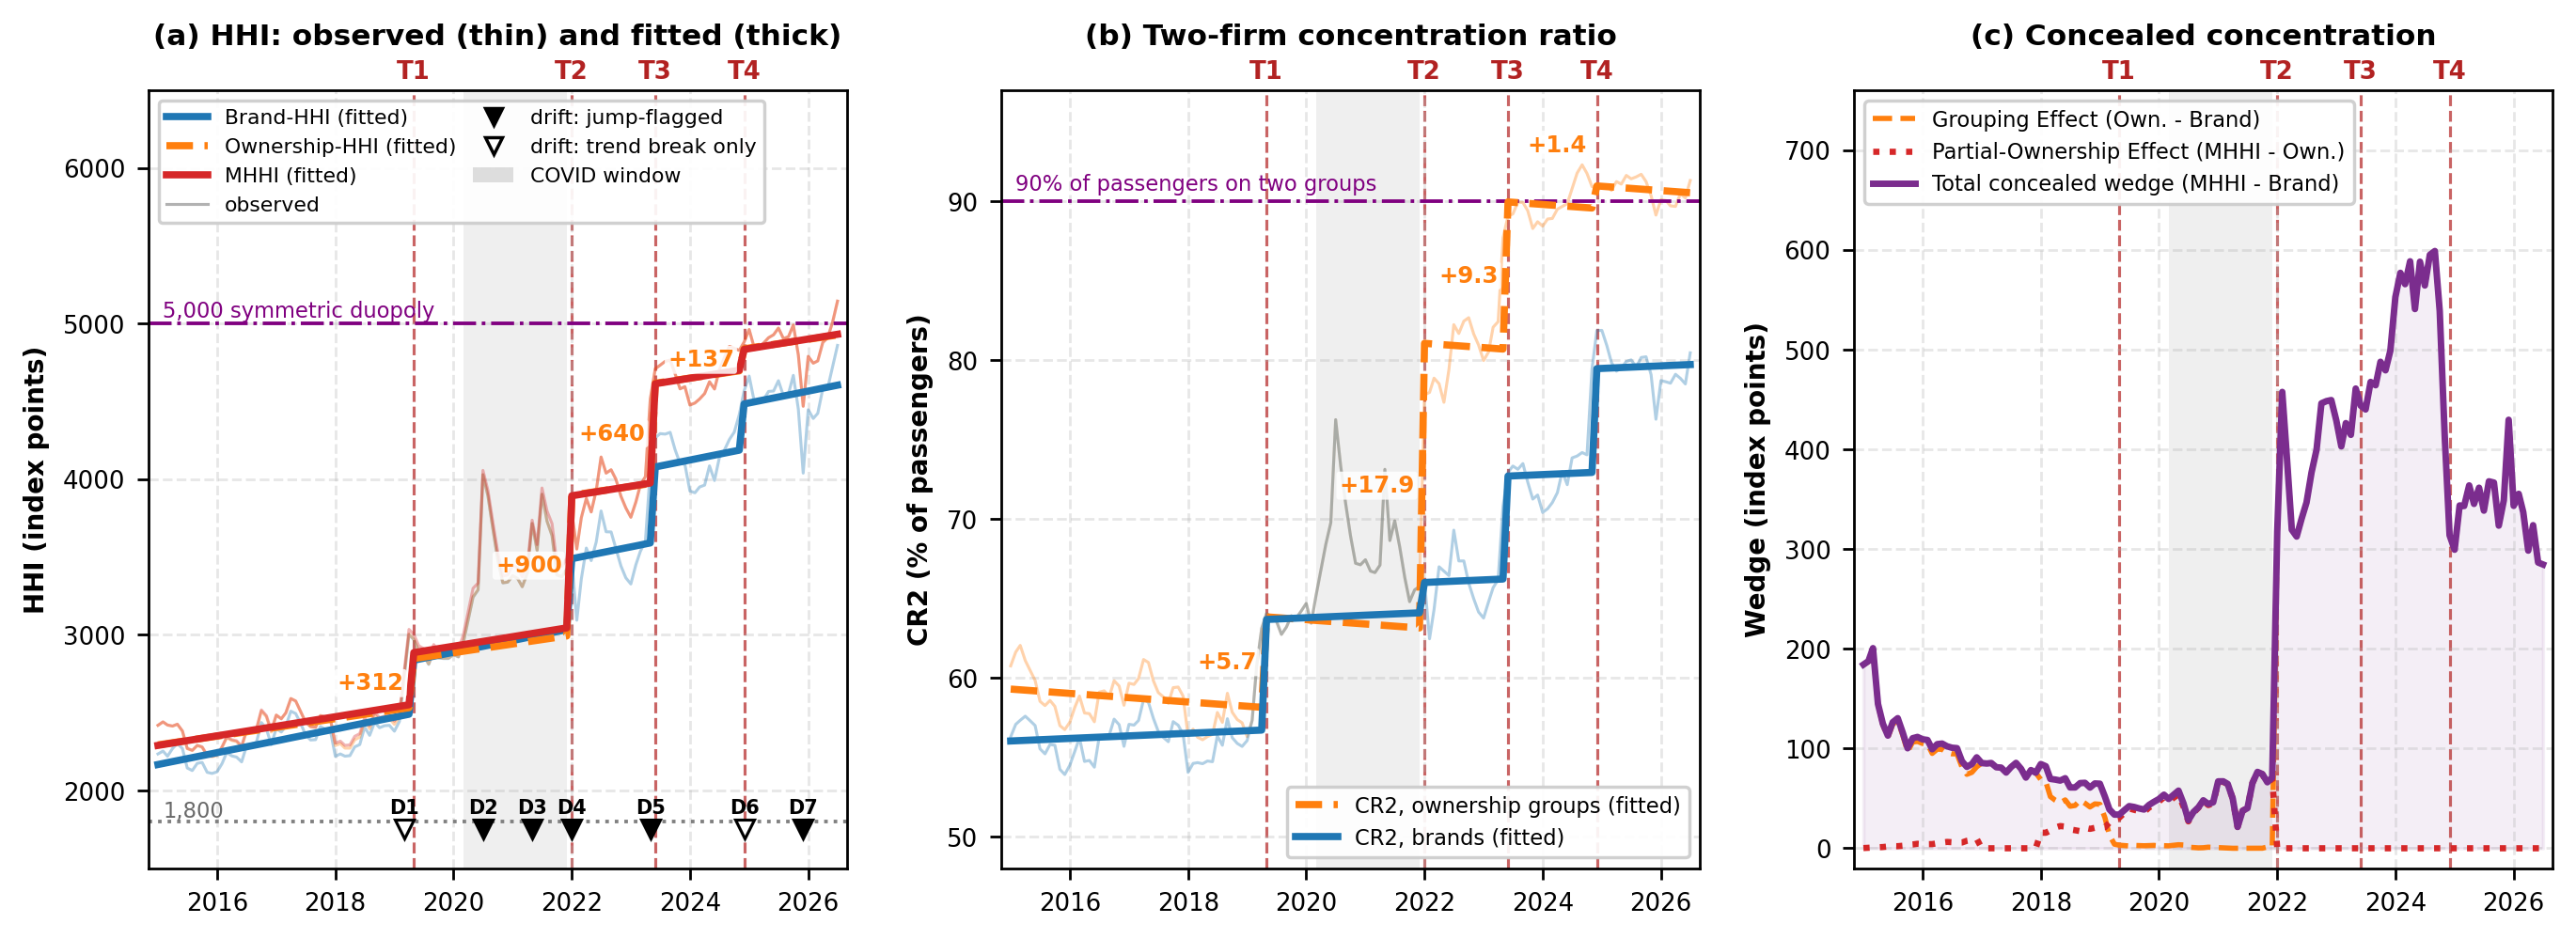
\includegraphics[width=\linewidth]{figures/o1_hhi.png}
\caption{O1: Interrupted time-series view of national concentration, January 2015--July 2026.}
\label{fig:o1-its}
\vspace{2pt}
\begin{minipage}{\linewidth}
\footnotesize\setstretch{1.1}
\textit{Note:} (a) Brand-, Ownership- and MHHI: observed (thin) and fitted (thick) values from Equation~O1.2, keeping the trend and the four event steps, with COVID and month-of-year terms netted out; figures beside each step are Ownership-HHI steps in points. (b) CR2 with its steps in percentage points. (c) Grouping Effect, Partial-Ownership Effect and their sum, the total concealed wedge. T1--T4: Jet exit, Tata acquisition, Go First exit, legal mergers. D1--D7: drift points (filled markers flagged by the jump detector). Grey band: COVID window.\par
\textit{Source:} DGCA monthly traffic via \href{https://github.com/mkubicek/india-aviation-stats/tree/16770ac59dae61ce7b80fd8bd67dd7f4cef280a6}{Kubicek (2026)}; authors' calculations.
\end{minipage}
\end{figure}

\clearpage
\section{Analysis and Results}
\subsection{O4: National concentration and dominance}
IndiGo and the Air India Group are the two largest ownership groups in all 20 months from December 2024 to July 2026, with IndiGo ranked first throughout. Their combined passenger share ranges from 89.13\% to 91.70\%, and the gap between them ranges from 30.01 to 43.39 percentage points. Thus the specified pair, CR2 and gap conditions occur together in every month of this period (Table~\ref{tab:o4-national-results}).

For each month, passengers are summed within the submitted ownership groups and shares are ranked afresh. We then count months meeting each condition using unrounded values. The full-series comparison covers 138 observed months from January 2015 to July 2026; April 2020 is missing. The focus period, December 2024--July 2026, has no missing months. Appendix~\ref{app:o4-national-calculations} gives the formulas and a worked example.

\begin{minipage}{\linewidth}
\captionsetup{font=small,labelfont=bf,justification=raggedright,singlelinecheck=false,hypcap=false}
\captionof{table}{National concentration conditions: full series and December 2024--July 2026.}
\label{tab:o4-national-results}
\centering
{\small\setstretch{1.1}\setlength{\tabcolsep}{4pt}\begin{tabular}{@{}lrrr@{}}
\toprule
 & \shortstack{Full series\\Months / 138} & \shortstack{Focus period\\Months / 20} & \shortstack{Focus period\\Range} \\
\midrule
IndiGo and AI Group lead & 59/138 & 20/20 & -- \\
CR2 $\geq 80\%$ & 48/138 & 20/20 & 89.13--91.70 \\
Share gap $>20$ pp & 120/138 & 20/20 & 30.01--43.39 \\
Fringe $\leq 20\%$ & 48/138 & 20/20 & 8.30--10.87 \\
Ownership HHI $>1{,}800$ & 138/138 & 20/20 & 4,468.57--5,144.35 \\
Pair, CR2 and gap jointly & 48/138 & 20/20 & -- \\
\bottomrule
\end{tabular}
\par}
\vspace{4pt}
{\footnotesize\setstretch{1.1}\raggedright\textit{Note:} Counts give months meeting the condition / observed months. AI Group means Air India Group. CR2 and fringe are passenger percentages; the gap is in percentage points (pp); HHI is in index points. Ranges use all 20 focus-period months. The final row combines the specified pair, CR2 $\geq80\%$ and gap $>20$ pp, the conditions in H5.\par
\textit{Source:} DGCA monthly airline traffic via \href{https://github.com/mkubicek/india-aviation-stats/tree/16770ac59dae61ce7b80fd8bd67dd7f4cef280a6}{Kubicek (2026)}; authors' calculations.\par}
\end{minipage}

Across the full series, the three conditions coincide in 48 of 138 observed months (34.8\%). High HHI alone is less selective: all 138 months exceed 1,800. The measures are related: fringe is $100-\mathrm{CR2}$, and CR2 $\geq80\%$ already implies HHI $\geq3{,}200$. They are therefore not independent tests. The $>20$ pp gap is the study-defined asymmetry threshold; these descriptive cutoffs are not a legal definition of duopoly.

Under the study's ownership convention, Vistara and AirAsia India are included in the Air India Group from January 2022, having been treated separately earlier. Combining previously separate groups raises ownership HHI even if their passenger shares are unchanged. The full-series comparison therefore reflects ownership consolidation as well as changes in passenger shares.

\clearpage
\subsection{O4: Route concentration and IndiGo dependence}
\textbf{Full-period results: April 2019--September 2026.}
Ownership-group frequency HHI exceeds 1,800 in 1,143 of the 1,150 retained airport-pair/month observations (99.39\%; Table~\ref{tab:o4-route-results}). Shares are calculated from approved scheduled flights, pooling both directions before grouping airlines by ownership. Each retained observation receives equal weight. Median CR2 is 80.00\%, the median share gap is 13.73 percentage points, and median fringe share is 20.00\%.

\begin{minipage}{\linewidth}
\captionsetup{font=small,labelfont=bf,justification=raggedright,singlelinecheck=false,hypcap=false}
\captionof{table}{Route concentration and IndiGo exposure, April 2019--September 2026.}
\label{tab:o4-route-results}
\centering
{\small\setstretch{1.1}\setlength{\tabcolsep}{5pt}\begin{tabular}{@{}lrr@{}}
\toprule
Condition & Observations & Share (\%) \\
\midrule
Ownership frequency HHI $>1{,}800$ & 1,143/1,150 & 99.39 \\
Group CR2 $\geq80\%$ & 583/1,150 & 50.70 \\
Group share gap $>20$ pp & 368/1,150 & 32.00 \\
IndiGo frequency share $\geq60\%$ & 79/1,150 & 6.87 \\
IndiGo is the sole scheduled operator & 0/1,150 & 0.00 \\
IndiGo and AI Group: unique top-two pair & 730/1,150 & 63.48 \\
Unique pair, CR2 and gap conditions jointly & 95/1,150 & 8.26 \\
Tie prevents a unique top-two pair & 58/1,150 & 5.04 \\
\bottomrule
\end{tabular}
\par}
\vspace{4pt}
{\footnotesize\setstretch{1.1}\raggedright\textit{Note:} The denominator is 1,150 retained observations from 20 selected airport pairs over 66 observed months. AI Group means Air India Group. The joint row requires this unique leading pair, CR2 $\geq80\%$ and gap $>20$ pp. A tie between second and third place prevents a unique pair; exchanging first and second does not change the pair. Conditions overlap. The 60\% exposure flag is study-defined.\par
\textit{Source:} DGCA approved domestic schedules; authors' calculations.\par}
\end{minipage}

High HHI does not establish the identity of the leading groups. IndiGo and Air India Group form the unique top-two pair in 730 observations (63.48\%); 95 observations (8.26\%) also meet the CR2 and gap conditions jointly. Other unique pairs include IndiGo--Vistara (99 observations) and IndiGo--Go First (83). There are 58 observations with a tie across the second-place boundary, reported separately rather than assigned to an arbitrary pair.

IndiGo's median frequency share is 43.60\%. It supplies at least 60\% of scheduled flights in 79 observations (6.87\%), all on Bengaluru--Kolkata, Chennai--Hyderabad or Bengaluru--Chennai. Across observed months, the percentage of available sampled pairs meeting this flag ranges from 0\% to 11.11\%; none has IndiGo as the sole scheduled operator. In December 2025, one of 19 available pairs meets the flag: Chennai--Hyderabad, at 78.10\%.

HHI exceeds 1,800 in 301 of 303 exact-endpoint-match observations (99.34\%), compared with 99.39\% in the full sample. Appendix~\ref{app:o4-route-calculations} gives the workings; Appendix~\ref{app:o4-route-checks} reports the subset comparisons and leading pairs. These findings describe scheduled-frequency concentration on selected major airport pairs; they are not passenger-share estimates or network-wide measures of IndiGo dependence.

\clearpage
\subsubsection*{Matched focus period: December 2024--July 2026}
During the focus period, IndiGo and Air India Group dominate the busiest sampled airport pairs, with other airlines collectively accounting for a relatively small share. However, the gap between the two leading groups is considerably smaller than nationally: route-level dominance is shared more evenly between IndiGo and Air India.

Table~\ref{tab:o4-route-focus} compares the same 20 calendar months nationally and on the selected routes. The top 20 pairs remain the submitted sample; the top 10 form a supplementary comparison using the first ten ranks in the same fixed 2025 passenger ranking. All 20 months are represented, with 184 of 200 possible pair-months retained for the top 10 and 350 of 400 for the top 20. Unavailable pair-months are excluded.

\begin{minipage}{\linewidth}
\captionsetup{font=small,labelfont=bf,justification=raggedright,singlelinecheck=false,hypcap=false}
\captionof{table}{National and route concentration during December 2024--July 2026.}
\label{tab:o4-route-focus}
\centering
{\small\setstretch{1.1}\setlength{\tabcolsep}{4pt}\begin{tabularx}{\linewidth}{|>{\raggedright\arraybackslash}X|r|r|r|}
\hline
\textbf{Measure} & \textbf{\shortstack{\strut National\\\strut Passenger data}} & \textbf{\shortstack{\strut Top 20\\\strut airport pairs\\\strut Scheduled flights}} & \textbf{\shortstack{\strut Top 10\\\strut airport pairs\\\strut Scheduled flights}} \\
\hline
IndiGo and AI Group are the unique top two & 20/20 & 328/350 & 184/184 \\
\hline
Median CR2 (\%) & 90.91 & 89.55 & 89.37 \\
\hline
Median share gap (pp) & 37.35 & 11.92 & 7.69 \\
\hline
Median fringe share (\%) & 9.09 & 10.45 & 10.63 \\
\hline
Leading pair, CR2 $\geq80\%$ and gap $>20$ pp, with IndiGo first & 20/20 & 50/350 & 9/184 \\
\hline
\end{tabularx}
\par}
\vspace{4pt}
{\footnotesize\setstretch{1.1}\raggedright\textit{Note:} National observations are months using passenger shares; route observations are airport-pair/months using scheduled-flight-frequency shares. Each observation has equal weight within its sample. Pair counts identify the two groups regardless of which ranks first. The joint row requires that pair, CR2 $\geq80\%$, gap $>20$ pp and IndiGo ranked first. AI Group means Air India Group; pp means percentage points.\par
\textit{Source:} DGCA monthly airline traffic via Kubicek (2026) and approved domestic schedules; authors' calculations.\par}
\end{minipage}

For the top 10 pairs, IndiGo and Air India are the unique leading pair in all 184 retained observations. Their median combined share is 89.37\%, leaving a median fringe share of 10.63\%. The median gap between the two leaders is 7.69 pp, compared with 37.35 pp nationally. IndiGo ranks first in 86 observations, Air India in 94, and they tie for first in four. The unique pair, CR2 and gap conditions hold with IndiGo leading in nine observations (4.89\%).

The top 20 give a similar pattern: the two groups form the unique leading pair in 328 of 350 observations (93.71\%), with median CR2 of 89.55\% and median gap of 11.92 pp. The IndiGo-led joint conditions hold in 50 observations (14.29\%). IndiGo supplies at least 60\% of scheduled flights in 26 observations (7.43\%) in the top 20 and none in the top 10. No retained observation in either focus-period sample has IndiGo as sole operator. Appendix~\ref{app:o4-route-focus} gives the coverage and calculation details. These comparisons distinguish IndiGo's lead over Air India from the leading pair's dominance over the smaller airlines.

\clearpage
\subsection{O4: Rivals' capacity buffer}
Rivals' unused capacity relative to IndiGo's passenger traffic falls from 9.79\% in December 2024 to 8.19\% in December 2025, a decline of 1.60 percentage points (Table~\ref{tab:o4-capacity-buffer}). December 2024 provides the same-calendar-month baseline. Unused capacity is each rival's available seat-kilometres (ASK) less its revenue passenger-kilometres (RPK), summed across all retained airlines other than IndiGo. Dividing that total by IndiGo's RPK and multiplying by 100 gives the buffer measure.

\begin{minipage}{\linewidth}
\captionsetup{font=small,labelfont=bf,justification=raggedright,singlelinecheck=false,hypcap=false}
\captionof{table}{Rivals' unused capacity relative to IndiGo's traffic, December comparison.}
\label{tab:o4-capacity-buffer}
\centering
{\small\setstretch{1.1}\setlength{\tabcolsep}{5pt}\begin{tabular}{@{}lrrr@{}}
\toprule
Measure & Dec 2024 & Dec 2025 & Change \\
\midrule
Rivals' ASK (billion seat-km) & 6.385 & 6.619 & +0.234 \\
Rivals' RPK (billion passenger-km) & 5.493 & 5.947 & +0.454 \\
Rivals' unused capacity (billion seat-km) & 0.892 & 0.672 & -0.220 \\
IndiGo RPK (billion passenger-km) & 9.113 & 8.208 & -0.905 \\
Buffer relative to IndiGo (\%) & 9.79 & 8.19 & -1.60 pp \\
\bottomrule
\end{tabular}
\par}
\vspace{4pt}
{\footnotesize\setstretch{1.1}\raggedright\textit{Note:} Rivals include nine retained airline brands in December 2024 and eight in December 2025; each is counted once. Changes are December 2025 minus December 2024, calculated before rounding. The buffer denominator is IndiGo's total monthly RPK; its change is in percentage points (pp).\par
\textit{Source:} DGCA monthly airline traffic via \href{https://github.com/mkubicek/india-aviation-stats/tree/16770ac59dae61ce7b80fd8bd67dd7f4cef280a6}{Kubicek (2026)}; authors' calculations.\par}
\end{minipage}

Rivals' offered capacity rises from 6.385 to 6.619 billion seat-km, but their passenger traffic increases by more in absolute terms, from 5.493 to 5.947 billion passenger-km. The unused gap consequently narrows from 0.892 to 0.672 billion seat-km, a reduction of 24.69\%. IndiGo's RPK also falls, from 9.113 to 8.208 billion passenger-km. The buffer ratio nevertheless declines because rivals' unused capacity falls proportionately more than its denominator.

The ratios correspond to 9.79 and 8.19 unused rival seat-km per 100 IndiGo passenger-km in the respective months. They compare the aggregate buffer with all IndiGo traffic, rather than the traffic affected by cancellations. Monthly national totals do not identify whether those unused seats matched passengers' routes and travel dates, or whether airlines could add flights using available aircraft, crews and airport slots. The calculation therefore measures the size of the aggregate buffer; it does not establish actual passenger accommodation. Appendix~\ref{app:o4-capacity-buffer} gives the airline-level contributions and worked calculations.

\clearpage
\subsection{O1: Event steps in concentration}
All four event steps are positive and significant in every model (Table~\ref{tab:o1-regression}). The Tata acquisition (900 vs.\ 449 points) and the Go First exit (640 vs.\ 482) are larger once brands are grouped by owner; the mergers are smaller (137 vs.\ 291) because they combined brands already grouped. The steps sum to 1,988 points for Ownership-HHI against 1,563 for Brand-HHI, so brand-level counting misses about a fifth of the event-driven rise. MHHI's Tata step is 56 points smaller than Ownership-HHI's because the partial-ownership wedge ends there. Re-dating the Jet and Go First steps to their drift months (March 2019, May 2023) lifts the Ownership-HHI sum to 2,211 and $R^2$ from 0.981 to 0.985 without changing the ranking.

\begin{minipage}{\linewidth}
\captionsetup{font=small,labelfont=bf,justification=raggedright,singlelinecheck=false,hypcap=false}
\captionof{table}{O1: Segmented regression of monthly concentration indices (Equation~O1.2).}
\label{tab:o1-regression}
\centering
{\small\setstretch{1.1}\setlength{\tabcolsep}{5pt}
\begin{tabular}{@{}lrrr@{}}
\toprule
Regressor & Brand HHI & Ownership HHI & MHHI \\
\midrule
Time trend (points per month) & 6.34\textsuperscript{**} (1.94) & 4.68\textsuperscript{*} (2.00) & 5.12\textsuperscript{*} (2.01) \\
Post-Jet exit (May 2019) & 340.83\textsuperscript{**} (78.99) & 311.51\textsuperscript{**} (79.12) & 330.33\textsuperscript{**} (79.50) \\
Post-Tata acquisition (Jan 2022) & 449.31\textsuperscript{**} (78.08) & 899.79\textsuperscript{**} (82.94) & 843.69\textsuperscript{**} (82.94) \\
Post-Go First exit (Jun 2023) & 481.99\textsuperscript{**} (50.45) & 640.03\textsuperscript{**} (56.18) & 632.96\textsuperscript{**} (55.21) \\
Post-legal mergers (Dec 2024) & 290.97\textsuperscript{**} (73.85) & 137.13\textsuperscript{*} (54.72) & 128.51\textsuperscript{*} (55.59) \\
COVID (Mar 2020--Dec 2021) & 517.84\textsuperscript{**} (44.59) & 543.41\textsuperscript{**} (45.53) & 547.56\textsuperscript{**} (45.25) \\
Sum of the four steps & 1{,}563 (222) & 1{,}988 (222) & 1{,}935 (223) \\
\midrule
$R^2$ & 0.972 & 0.981 & 0.981 \\
Durbin--Watson & 0.92 & 0.93 & 0.94 \\
\bottomrule
\end{tabular}\par}
\vspace{4pt}
{\footnotesize\setstretch{1.1}\raggedright\textit{Note:} Newey--West standard errors (12 lags) in parentheses; $n=138$. \textsuperscript{*}$p<0.05$, \textsuperscript{**}$p<0.01$. Constant and eleven month-of-year dummies included. Breusch--Godfrey (12 lags) rejects no autocorrelation and the ADF test rejects a unit root in the residuals ($p<0.001$ in all three models).\par
\textit{Source:} DGCA monthly airline traffic via \href{https://github.com/mkubicek/india-aviation-stats/tree/16770ac59dae61ce7b80fd8bd67dd7f4cef280a6}{Kubicek (2026)}; authors' calculations.\par}
\end{minipage}

CR2 on ownership groups averages 72.0\%, rising from 58.7\% to 90.7\% across the periods and reaching 91.3\% in July 2026 (IndiGo 67.4\%, Air India Group 24.0\%). Its steps are $+5.7$, $+17.9$, $+9.3$ and $+1.4$ points (total 34.4); at brand level the Tata step is only 1.9 and the merger step 6.5. January 2022 is its largest monthly move ($+12.1$). CR2 and Ownership-HHI correlate at 0.983 in levels but 0.794 in monthly changes (Appendix~\ref{app:o1-cr2}).

\clearpage
\section{Discussion}
\subsection{O4: Economic interpretation}
\textbf{National asymmetry within a concentrated oligopoly.} During December 2024--July 2026, IndiGo and Air India Group carry a median 90.91\% of national passengers, leaving a median 9.09\% to the other airlines (Table~\ref{tab:o4-route-focus}). IndiGo's median lead over Air India Group is 37.35 percentage points. This pattern is consistent with an asymmetric duopoly and a small competitive fringe. Strategic interdependence is central to such a structure: capacity or pricing decisions by either large group can affect the demand faced by its rival. The shares establish the relative scale of the groups, while their actual pricing and output strategies remain unobserved.

\textbf{Market definition and route-level alternatives.} The alternatives available to a passenger depend on the journey: a seat on another airport pair does not automatically meet the same travel need. On the busiest ten sampled pairs, IndiGo and Air India are the two largest groups in all 184 retained focus-period observations. Their median combined scheduled-flight share is 89.37\%, leaving a relatively small fringe, but the median gap between the leaders is only 7.69 pp. The twenty-pair sample gives the same broad pattern. Thus the route evidence corroborates two-group dominance over the smaller airlines, while showing a more balanced division between IndiGo and Air India. National passenger shares and route scheduled-flight shares are different measures; they do not isolate the role of network coverage or establish route profitability.

\textbf{Short-run supply constraints and resilience.} Rival airlines cannot expand replacement service immediately simply because additional demand arises. Aircraft, crews and airport access constrain short-run supply, while unused seats must match passengers' routes and travel dates. The decline in rivals' unused capacity relative to IndiGo's traffic, from 9.79\% to 8.19\%, indicates less aggregate headroom in December 2025 (Table~\ref{tab:o4-capacity-buffer}). For contingency planning, the existence of another large airline therefore does not by itself establish readily available substitute capacity. The buffer describes unused seat-distance relative to IndiGo's total traffic; it measures neither actual accommodation of disrupted passengers nor short-run supply elasticity.

Concentration describes market structure, while competitive conduct and economic performance require additional evidence. A large share can reflect efficiency advantages as well as weaker competitive pressure. Without fare and cost data, these results cannot distinguish those explanations or establish effects on markups, profits or passenger welfare.

\clearpage
\subsection{O4: Hypotheses revisited}
All three O4 hypotheses are supported within their specified samples and comparison periods (Table~\ref{tab:o4-hypotheses}). These outcomes assess the descriptive conditions stated in Assignment~2; they are not statistical significance tests or causal estimates.

\begin{minipage}{\linewidth}
\captionsetup{font=small,labelfont=bf,justification=raggedright,singlelinecheck=false,hypcap=false}
\captionof{table}{O4 hypotheses: outcomes and supporting evidence.}
\label{tab:o4-hypotheses}
\centering
{\small\setstretch{1.1}\setlength{\tabcolsep}{5pt}\begin{tabular}{@{}>{\raggedright\arraybackslash}p{0.35\linewidth}>{\raggedright\arraybackslash}p{0.15\linewidth}>{\raggedright\arraybackslash}p{0.43\linewidth}@{}}
\toprule
Hypothesis & Outcome & Evidence \\
\midrule
\textbf{H5: National.} IndiGo and AI Group are the top two in every month, Dec 2024--Jul 2026, with CR2 $\geq80\%$ and gap $>20$ pp. & Supported & 20/20 months; minimum CR2 89.13\%; minimum gap 30.01 pp. Table~\ref{tab:o4-national-results}. \\
\addlinespace[6pt]
\textbf{H6: Routes.} Ownership-adjusted frequency HHI $>1{,}800$ in more than half of available observations for the selected 20 pairs. & Supported & 1,143/1,150 pair-months (99.39\%) exceed 1,800. Table~\ref{tab:o4-route-results}. \\
\addlinespace[6pt]
\textbf{H7: Buffer.} Rivals' unused capacity relative to IndiGo RPK is lower in Dec 2025 than Dec 2024. & Supported & 9.7905\% to 8.1865\%; change -1.6040 pp. Table~\ref{tab:o4-capacity-buffer}. \\
\bottomrule
\end{tabular}
\par}
\vspace{4pt}
{\footnotesize\setstretch{1.1}\raggedright\textit{Note:} AI Group means Air India Group; pp means percentage points. H6 uses the full April 2019--September 2026 route sample. The H7 denominator is IndiGo's total monthly RPK.\par
\textit{Source:} Authors' calculations from the Section~5 data.\par}
\end{minipage}

H6 concerns high route concentration, rather than requiring IndiGo to lead Air India by a large margin on every pair. The focus-period comparison therefore qualifies the broader description of asymmetry without contradicting H6: the two groups dominate the busiest sampled pairs, but their scheduled-flight shares are more evenly balanced than their national passenger shares. H7 supports a smaller aggregate buffer, without establishing how many disrupted passengers could actually be accommodated.

\textcite{kumari2026soaring} find that operational efficiency, particularly passenger load factor, matters for airline profitability alongside market structure. Our results preserve that distinction: H5 and H6 establish concentration under the specified measures, while the capacity comparison adds evidence about unused seat-distance. The route results extend the national perspective by distinguishing dominance over the fringe from the gap between the two leaders; they do not replicate the paper's profitability tests or establish collusion.

\textcite{gupta2025antitrust} warn that dependence on a dominant airline can magnify disruption risks. Our capacity comparison adds descriptive evidence of a declining buffer, without establishing that concentration caused the disruption or prevented recovery.

\clearpage
\subsection{O1: Economic interpretation}
\textbf{From oligopoly towards asymmetric duopoly.} Ownership-HHI rose from a mean of 2,408 before the Jet Airways exit to 4,877 after the mergers, equivalent to falling from 4.2 to 2.1 equal-sized airlines; nine in ten passengers now fly IndiGo or the Air India Group. Concentration never left the highly concentrated band, so what changed is the distance above it, and it changed in steps tied to exits and changes of control rather than through gradual drift.

\textbf{Ownership matters more than brands.} The Tata acquisition is the largest step (about 900 points), and half of it is the Grouping Effect: brands that remained separate in DGCA reports came under one owner. Brand shares alone would understate that step by half. Partial ownership is small: the wedge averages 23 points before 2022 and never exceeds 77.

\textbf{Course lenses.} Read through structure--conduct--performance \parencite{gandhi2026marketstructure}, the rise signals greater potential market power. Under Cournot competition the industry Lerner index is HHI$/|\varepsilon|$; with $|\varepsilon|=1.5$ the permanent drifts D1 and D5 imply margins 3.5 and 4.6 points higher. This is an implication of structure, not a measured markup. IndiGo's large aircraft orders act as Stackelberg-style capacity commitments, and its share rose from 57.5\% to 63.2\% across D5 and was held. Both exits occurred with HHI already above 1,800, and Akasa Air's entry in August 2022 was followed only by a slow fall of about 390 points over six months, so entry has not offset consolidation.

\clearpage
\subsection{O1: Hypotheses revisited}
\textbf{H1 (lasting event steps): supported for the Jet, Tata and Go First events; weak for the mergers.} Their drifts ($+531$, $+367$ and $+693$ points) never reverse, and their regression steps are significant at 1\%. D6 adds only 54 points and is not flagged by the jump detector; its regression step is 137 points ($t=2.5$). All four steps stay significant at 6 or 18 lags and with COVID months dropped ($t\geq2.2$), and CR2 agrees. The transient drifts D2, D3 and D7 reverse, so a lasting rise requires an exit or a change of control.

\textbf{H2 (partial-ownership wedge): partially supported, economically negligible.} MHHI exceeds Ownership-HHI before January 2022, but the wedge averages 22.9 points (0.8\% of Ownership-HHI, maximum 2.2\%) and disappears at D4. It changes no month's concentration classification (Appendix~\ref{app:o1-wedge}).

\textbf{Grouping gap.} Ownership-HHI is never below Brand-HHI. The gap moves only at the reclassification drifts, widening by 316 points at D4 and narrowing by 100 at D6, against $-27$ and $+29$ at the exits (Appendix~\ref{app:o1-wedge}).

These outcomes describe dated level shifts in national structure; they are not causal estimates of the events' effects on fares, profits or passengers.

\section{Implications and Recommendations}
Discuss the implications of the findings for the relevant stakeholders.

Depending on the topic, these may include:
\templatebullet{Firms and managers}
\templatebullet{Consumers}
\templatebullet{Regulators}
\templatebullet{Policymakers}
\templatebullet{Industry participants}
Provide 2--3 specific recommendations where appropriate. Recommendations should follow from the findings of the study.

\clearpage
\section{Limitations}
\subsection{O4: Measurement, coverage and interpretation}
\textbf{Scheduled frequency versus passengers carried.} Route concentration uses approved scheduled-flight frequencies, while national concentration uses passenger shares. Flights differ in aircraft size and occupancy, and schedules may differ from actual operations. Consequently, the smaller IndiGo--Air India gap on busy airport pairs describes scheduled frequency; it does not establish an equally balanced division of route passengers. The findings also cannot determine how much of the national--route difference comes from network coverage, aircraft size or occupancy. Airline-by-route passenger and operated-flight data would allow a closer comparison.

\textbf{Incomplete coverage and selected airport pairs.} The sample fixes the twenty busiest pairs by 2025 passengers. In the matched focus period, 350 of 400 possible top-20 pair-months are available; the top-ten comparison retains 184 of 200. These observations need not represent missing pair-months or smaller routes elsewhere in the network. Source-quality screens and the two documented TruJet-related exclusions improve consistency but cannot detect every missing airline filing. Although 99.34\% of exact-endpoint-match observations exceed HHI 1,800, compared with 99.39\% overall, this does not establish complete coverage or random missingness.

\textbf{Aggregate capacity buffer.} The fall from 9.79\% to 8.19\% compares monthly unused rival seat-kilometres with all IndiGo passenger-kilometres, rather than the traffic affected by cancellations. It does not show whether unused seats were available on the required routes and dates, or whether additional aircraft, crews and airport slots could be deployed. The two-December comparison is descriptive and cannot establish the cause of the smaller buffer or actual passenger accommodation. Assessing recovery would require disruption-specific demand and route/date-specific available capacity.

\textbf{Ownership conventions and limits to inference.} The January 2022 ownership regrouping mechanically changes concentration, so movements around that date cannot be attributed entirely to passenger redistribution. April 2020 is missing nationally and is not imputed; pandemic-era changes also complicate comparisons across the full series. The gap and IndiGo-exposure thresholds are study-defined descriptive flags. The observed persistence of the national pattern does not establish that it will continue beyond July 2026. Without fare, marginal-cost and recovery data, concentration and buffer measures cannot establish collusion, fare effects, profitability or passenger harm.

\clearpage
\subsection{O1: Measurement and inference}
\textbf{Steps, not causes.} The $\gamma_k$ are dated level shifts with autocorrelated residuals. Akasa Air's ramp-up, SpiceJet's decline and slot reallocations are absorbed into the steps and trend, and four events allow no counterfactual. Drift detectors locate changes; they do not identify causes.

\textbf{Coarse controls and data gaps.} A single indicator covers March 2020--December 2021. AirAsia India is missing from the source in 2017, so headline HHI is overstated by about 165--171 points in those months, and the zero wedge then is a data gap.

\textbf{Assembled ownership stakes.} MHHI relies on three press-sourced points, an undated step from 49\% to 51\% in AirAsia India, and modelled control; only the Tata, Singapore Airlines, AirAsia Investment and Telestra stakes are included.

\textbf{Grouping and scale.} Alliance Air stays separate before 2022 (grouping it would add 22.5 points on average). The analysis is national, shares are based on passengers rather than capacity, and only 20 months follow the mergers. Without fares or costs, the indices describe market structure, not market power.

\section{Conclusion}
Summarise the research question, main findings, key economic interpretation, and main implications.

\newpage
\nocite{kubicek2026aviationstats,dgcaDomesticSchedules}
\printbibliography[title={References}]

\newpage
\appendix
\section{Variable Dictionary}
\label{app:o4-dictionary}
\subsection{O4: Observation keys and inputs}
The dictionary covers the inputs, measures and flags used in O4's reported analysis and supporting outputs. National observations are market-months; route observations are airport-pair/months. Detailed extraction-column and CSV documentation accompanies the code repository.

\begin{minipage}{\linewidth}
\captionsetup{font=small,labelfont=bf,justification=raggedright,singlelinecheck=false,hypcap=false}
\captionof{table}{O4 observation keys and input variables.}
\label{tab:o4-dictionary-inputs}
\centering
{\footnotesize\setstretch{1.0}\setlength{\tabcolsep}{4pt}\begin{tabular}{@{}>{\raggedright\arraybackslash}p{0.24\linewidth}>{\raggedright\arraybackslash}p{0.59\linewidth}>{\raggedright\arraybackslash}p{0.12\linewidth}@{}}
\toprule
Variable / key & Meaning and construction & Unit \\
\midrule
Month & Calendar month. National and capacity CSVs use a first-of-month date (YYYY-MM-01); route CSVs use YYYY-MM. & Month \\
\addlinespace[5pt]
Airline brand & Standardised operating-brand label. Positive-passenger scheduled-domestic records form the national and capacity samples. & Category \\
\addlinespace[5pt]
Ownership group & Airline brands combined under the study's common-ownership convention; group passengers or flights are summed before shares are calculated. & Category \\
\addlinespace[5pt]
Airport pair & Unordered pair of airport codes, with both directions pooled. A pair in one month is one route observation. GOI and GOX remain separate airports. & Identifier \\
\addlinespace[5pt]
2025 route passengers and rank & Passenger journeys summed over both directions and all twelve months of 2025. Descending totals fix the top-twenty selection and its top-ten subset for every study month. These data have no airline breakdown. & Journeys; rank \\
\addlinespace[5pt]
National passengers, $P_{gt}$ & Passenger journeys carried by ownership group $g$ in month $t$, summed over retained airline brands. These are journeys, not unique travellers. & Journeys \\
\addlinespace[5pt]
Scheduled flights, $f_{grt}$ & Approved scheduled departures for group $g$, pair $r$, month $t$, pooling both directions. Weekdays and validity dates are expanded; each airline/flight/date/directed-leg event is counted once. & Flights \\
\addlinespace[5pt]
ASK and RPK & ASK is seats offered times distance; RPK is revenue passengers carried times distance. Reported source values are in thousands; dividing by 1,000,000 expresses them in billions. & Seat-km; passenger-km \\
\bottomrule
\end{tabular}
\par}
\vspace{4pt}
{\footnotesize\setstretch{1.0}\raggedright\textit{Source:} Authors' definitions based on the DGCA inputs used in O4.\par}
\end{minipage}

\textbf{Ownership convention.} Air India and Air India Express are combined throughout, as are Jet Airways and JetLite. Vistara and AirAsia India/AIX Connect also join Air India Group from January 2022; they are separate earlier. Other brands, including Alliance Air, remain separate.

\textbf{Periods and sample flags.} National: January 2015--July 2026, excluding missing April 2020. Routes: available April 2019--September 2026. Focus period: December 2024--July 2026. Top-ten membership selects fixed ranks 1--10. The buffer compares December 2024 with December 2025.

\clearpage
\subsection{O4: Constructed measures}
In Table~\ref{tab:o4-dictionary-measures}, $g$ denotes an ownership group, $r$ an airport pair and $t$ a month. Shares $s$ are percentages, and subscripts $(1)$ and $(2)$ identify the largest and second-largest shares in the observation. Percentage points are abbreviated pp.

\begin{minipage}{\linewidth}
\captionsetup{font=small,labelfont=bf,justification=raggedright,singlelinecheck=false,hypcap=false}
\captionof{table}{O4 constructed measures and units.}
\label{tab:o4-dictionary-measures}
\centering
{\footnotesize\setstretch{1.0}\setlength{\tabcolsep}{4pt}\begin{tabular}{@{}>{\raggedright\arraybackslash}p{0.24\linewidth}>{\raggedright\arraybackslash}p{0.59\linewidth}>{\raggedright\arraybackslash}p{0.12\linewidth}@{}}
\toprule
Measure & Definition & Unit \\
\midrule
National group share & $s_{gt}=100P_{gt}/\sum_gP_{gt}$, using monthly passenger journeys. & \% \\
\addlinespace[5pt]
Route group share & $s_{grt}=100f_{grt}/\sum_gf_{grt}$, using scheduled flights on the pair in that month. & \% \\
\addlinespace[5pt]
Ownership / brand HHI & $\sum s^2$, with shares on the 0--100 scale. Ownership HHI sums squared group shares; brand HHI instead treats each operating brand separately. & Index points \\
\addlinespace[5pt]
CR2 & $s_{(1)}+s_{(2)}$, the combined share of the two largest groups, ranked afresh for each observation. & \% \\
\addlinespace[5pt]
Leader--rival gap & $s_{(1)}-s_{(2)}$. Nonnegative; this compares the two largest groups, whichever group leads. & pp \\
\addlinespace[5pt]
Fringe share & $100-\mathrm{CR2}$. Combined share of all groups outside the leading pair. & \% \\
\addlinespace[5pt]
IndiGo / AI frequency share & Each named group's scheduled flights divided by all scheduled flights on the pair in that month, times 100. & \% \\
\addlinespace[5pt]
Signed IndiGo--AI gap & IndiGo's frequency share minus Air India Group's. Unlike the leader--rival gap, it can be negative; retained in the focus-period CSV. & pp \\
\addlinespace[5pt]
Unused rival capacity, $U_t$ & $\sum_{j\ne I}(\mathrm{ASK}_{jt}-\mathrm{RPK}_{jt})$, where $I$ is IndiGo. Every retained rival brand is counted once. & Seat-km \\
\addlinespace[5pt]
Buffer relative to IndiGo, $B_t$ & $100U_t/\mathrm{RPK}_{It}$. The denominator is all IndiGo monthly RPK, not rivals' ASK or cancellation-affected traffic. & \% \\
\addlinespace[5pt]
Buffer change / unused-capacity change & $B_{2025}-B_{2024}$ is the buffer change in pp. $100(U_{2025}/U_{2024}-1)$ is the percentage change in unused capacity, comparing the two Decembers. & pp; \% \\
\addlinespace[5pt]
Exposure / condition percentages & Monthly exposure: 100 times flagged pairs divided by retained pairs that month. Pooled percentages: 100 times qualifying pair-months divided by all retained pair-months in the stated sample. & \% \\
\addlinespace[5pt]
Summary statistics & Means, medians, sample standard deviations and ranges use equally weighted observations within the stated sample. Route quartiles use linear interpolation. & Measure's unit \\
\bottomrule
\end{tabular}
\par}
\vspace{4pt}
{\footnotesize\setstretch{1.0}\raggedright\textit{Source:} Definitions implemented in the O4 analysis code.\par}
\end{minipage}

All calculations precede display rounding. Pooled route summaries weight pair-months equally; pairs with more retained months contribute more observations. HHI ranges from zero to 10,000 in principle. Source and display capacity units differ only in scale; missing values are not zero.

\clearpage
\subsection{O4: Flags, coverage and missingness}
Boolean flags are saved as True/False. Table~\ref{tab:o4-dictionary-flags} defines the conditions behind the reported counts. These descriptive flags do not identify pricing conduct or constitute independent tests of duopoly.

\begin{minipage}{\linewidth}
\captionsetup{font=small,labelfont=bf,justification=raggedright,singlelinecheck=false,hypcap=false}
\captionof{table}{O4 analytical flags and source-quality conventions.}
\label{tab:o4-dictionary-flags}
\centering
{\footnotesize\setstretch{1.0}\setlength{\tabcolsep}{4pt}\begin{tabular}{@{}>{\raggedright\arraybackslash}p{0.24\linewidth}>{\raggedright\arraybackslash}p{0.59\linewidth}>{\raggedright\arraybackslash}p{0.12\linewidth}@{}}
\toprule
Flag / convention & Rule and interpretation & Unit \\
\midrule
Concentration flags & True when ownership HHI $>1{,}800$, CR2 $\geq80\%$, gap $>20$ pp or fringe $\leq20\%$, respectively. CR2 and fringe conditions are equivalent; gap $>20$ pp is study-defined. & Boolean \\
\addlinespace[5pt]
IndiGo exposure / sole operator & Exposure is True when IndiGo supplies $\geq60\%$ of scheduled flights (study-defined). Sole operator is True only when all scheduled flights belong to IndiGo. & Boolean \\
\addlinespace[5pt]
Leading-group identities and ties & Groups rank by passengers nationally or flights on each pair-month. Alphabetical ordering resolves ties for display. A route tie across ranks two and three prevents a unique top-two pair; a two-way first-place tie alone does not. & Categories; Boolean \\
\addlinespace[5pt]
IndiGo--AI leading-pair flag & True when the top two are IndiGo and Air India Group, regardless of order. The route ``unique pair'' flag also requires no tie across ranks two and three. & Boolean \\
\addlinespace[5pt]
Joint concentration flags & H5 combines the national pair flag with CR2 $\geq80\%$ and gap $>20$ pp. The route joint flag applies those conditions to the unique pair; the IndiGo-led variant additionally requires IndiGo to lead. H6 counts observations using only the HHI flag. & Boolean \\
\addlinespace[5pt]
First-place leadership flags & IndiGo or AI is a unique leader only if its share strictly exceeds every rival's. First-place ties are counted separately, including in focus-period leadership totals. & Boolean \\
\addlinespace[5pt]
Endpoint discrepancy / exact match & Discrepancy is 100 times the sum of absolute airline departure--arrival count differences divided by total departures, pooling directions. Exact match is True only if each airline's two totals agree. & \%; Boolean \\
\addlinespace[5pt]
Retained pair-month / available pairs & Retention requires full-month source coverage, endpoint discrepancy $\leq5\%$ and at least ten qualifying pairs in the full twenty-pair panel that month, after exclusions. HYD--MAA in February--March 2022 is excluded. Available pairs count retained observations in the month. & Boolean; count \\
\addlinespace[5pt]
Capacity validity & A valid positive-passenger record has ASK $>0$ and $0\leq\mathrm{RPK}\leq\mathrm{ASK}$. Invalid records remain flagged without imputation; the buffer calculation requires every selected December record to be valid. & Category \\
\bottomrule
\end{tabular}
\par}
\vspace{4pt}
{\footnotesize\setstretch{1.0}\raggedright\textit{Source:} Rules implemented in the O4 preparation and analysis code.\par}
\end{minipage}

\textbf{Missingness.} Unavailable or excluded pair-months are absent from analysis tables and blank in the heatmap matrix (grey in the figure). Zero available pairs means no retained data, not zero flights. Coverage checks do not prove all filings are present. Observed zero gaps, fringe shares or exposure counts remain valid values. Preparation and workings are in Appendix~\ref{app:o4-route-preparation}.

\clearpage
\subsection{O1: Variables and measures}
\label{app:o1-dictionary}
Shares are passenger percentages within each market-month, so each HHI ranges from near zero to 10,000. $s_i$ denotes a brand share, $S_g$ an ownership-group share and $S_{(1)}, S_{(2)}$ the largest and second-largest group shares.

\begin{minipage}{\linewidth}
\captionsetup{font=small,labelfont=bf,justification=raggedright,singlelinecheck=false,hypcap=false}
\captionof{table}{O1: Variables, construction and units.}
\label{tab:o1-dictionary}
\centering
{\footnotesize\setstretch{1.0}\setlength{\tabcolsep}{4pt}
\begin{tabular}{@{}p{3.6cm}p{9.2cm}p{1.9cm}@{}}
\toprule
Variable & Definition and construction & Unit \\
\midrule
\multicolumn{3}{@{}l}{\textit{Dependent (outcome) variables}} \\
Brand-HHI & $\sum_i s_i^2$, each operating brand treated as a firm & points \\
Ownership-HHI & $\sum_g S_g^2$, brands summed into ownership groups & points \\
MHHI & Ownership-HHI plus the partial-ownership term of Equation~O1.1b, with stakes $\beta$ from Table~\ref{tab:o1-stakes} and proportional control & points \\
CR2 & $S_{(1)}+S_{(2)}$, combined share of the two largest ownership groups; a brand-level version uses the two largest brands & \% \\
Grouping Effect & Ownership-HHI minus Brand-HHI & points \\
Partial-Ownership Effect & MHHI minus Ownership-HHI (the wedge) & points \\
Effective number of firms & $10{,}000/\text{Ownership-HHI}$ & firms \\
Share gap & $S_{(1)}-S_{(2)}$ & pp \\
Fringe share & $100-\mathrm{CR2}$ & \% \\
IndiGo ratio & IndiGo's share divided by the second-largest group's share & ratio \\
\midrule
\multicolumn{3}{@{}l}{\textit{Main explanatory variables}} \\
Post-event indicators & 1 from the first full month after each event: Jet exit (May 2019), Tata acquisition (Jan 2022), Go First exit (Jun 2023), legal mergers (Dec 2024) & 0/1 \\
Time trend & Calendar month index (January 2015 $=1$; April 2020 keeps its index) & months \\
\midrule
\multicolumn{3}{@{}l}{\textit{Control variables}} \\
COVID period & 1 for March 2020 to December 2021 & 0/1 \\
Month of year & Eleven month indicators (January is the base) & 0/1 \\
\bottomrule
\end{tabular}\par}
\vspace{4pt}
{\footnotesize\setstretch{1.0}\raggedright\textit{Source:} Definitions implemented in the O1 analysis code (\texttt{o1\_analysis.py}).\par}
\end{minipage}

\clearpage
\section{Additional Tables and Figures}
\label{app:o4-national-summary}
\begin{minipage}{\linewidth}
\captionsetup{font=small,labelfont=bf,justification=raggedright,singlelinecheck=false,hypcap=false}
\captionof{table}{National concentration: descriptive statistics, January 2015--July 2026.}
\label{tab:o4-national-summary}
\centering
{\small\setstretch{1.1}\begin{tabular}{@{}lrrrrr@{}}
\toprule
Measure & Mean & Median & Std. dev. & Minimum & Maximum \\
\midrule
Ownership HHI (points) & 3,446.95 & 3,367.72 & 991.68 & 2,216.18 & 5,144.35 \\
CR2 (\%) & 71.97 & 66.90 & 13.43 & 56.09 & 92.30 \\
Share gap (pp) & 30.92 & 32.24 & 8.87 & 11.11 & 49.87 \\
Fringe share (\%) & 28.03 & 33.10 & 13.43 & 7.70 & 43.91 \\
\bottomrule
\end{tabular}
\par}
\vspace{4pt}
{\footnotesize\setstretch{1.1}\raggedright\textit{Note:} Each measure has 138 observed months, weighted equally. April 2020 is missing and is not imputed. HHI uses squared ownership-group percentage shares; CR2 adds the largest two shares, the gap subtracts the second from the first, and fringe share is $100-\mathrm{CR2}$. Standard deviations use the sample formula; pp means percentage points.\par
\textit{Source:} DGCA monthly airline traffic via Kubicek (2026); authors' calculations.\par}
\end{minipage}

\clearpage
\subsection{O1: Summary statistics and drift points}
\label{app:o1-tables}
\begin{minipage}{\linewidth}
\captionsetup{font=small,labelfont=bf,justification=raggedright,singlelinecheck=false,hypcap=false}
\captionof{table}{O1: Descriptive statistics, January 2015--July 2026.}
\label{tab:o1-summary}
\centering
{\small\setstretch{1.1}\setlength{\tabcolsep}{5pt}
\begin{tabular}{@{}lrrrrl@{}}
\toprule
Series & Mean & SD & Min & Max & Unit \\
\midrule
Brand-HHI & 3{,}248.9 & 856.3 & 2{,}109.1 & 4{,}859.8 & points \\
Ownership-HHI & 3{,}447.0 & 991.7 & 2{,}216.2 & 5{,}144.4 & points \\
MHHI (proportional control) & 3{,}460.7 & 987.2 & 2{,}220.7 & 5{,}144.4 & points \\
CR2 & 72.0 & 13.4 & 56.1 & 92.3 & \% \\
Effective number of firms & 3.15 & 0.89 & 1.94 & 4.51 & firms \\
Share gap & 30.9 & 8.9 & 11.1 & 49.9 & pp \\
Fringe share & 28.0 & 13.4 & 7.7 & 43.9 & \% \\
IndiGo ratio & 2.68 & 0.92 & 1.44 & 6.47 & ratio \\
\bottomrule
\end{tabular}\par}
\vspace{4pt}
{\footnotesize\setstretch{1.1}\raggedright\textit{Note:} 138 observed market-months, equally weighted; April 2020 is missing and not imputed. Brand- and Ownership-HHI nearly coincide between mid-2019 and January 2022 (mean gap 1.4 points) and separate afterwards; MHHI lies within 80 points of Ownership-HHI throughout.\par
\textit{Source:} DGCA monthly airline traffic via Kubicek (2026); authors' calculations.\par}
\end{minipage}

\vspace{1.2em}
\begin{minipage}{\linewidth}
\captionsetup{font=small,labelfont=bf,justification=raggedright,singlelinecheck=false,hypcap=false}
\captionof{table}{O1: Drift points in the concentration indices.}
\label{tab:o1-drift}
\centering
{\footnotesize\setstretch{1.0}\setlength{\tabcolsep}{3pt}
\begin{tabular}{@{}lp{2.0cm}rrrrp{3.6cm}p{3.3cm}@{}}
\toprule
ID & Window & $\Delta$Br. & $\Delta$Own. & $\Delta$MHHI & $\Delta$CR2 & Largest share movers (pp) & Reading \\
\midrule
D1 & Feb--Apr 2019 & $+558$ & $+531$ & $+540$ & $+5.8$ & Jet group $-10.4$; IndiGo $+6.4$ & Share shift (Jet exit); permanent \\
D2 & Jun--Jul 2020 & $+741$ & $+739$ & $+724$ & $+6.5$ & IndiGo $+7.6$; Air India Group $-3.3$ & Share shift (post-lockdown restart); retraced by Nov 2020 \\
D3 & Apr--May 2021 & $+321$ & $+321$ & $+292$ & $+6.0$ & Air India Group $+6.1$; AirAsia India $-3.2$ & Share shift (second COVID wave); retraced by Oct 2021 \\
D4 & Dec 2021--Jan 2022 & $+51$ & $+367$ & $+297$ & $+12.1$ & Air India Group $+13.9$ (Vistara $-7.7$, AirAsia India $-6.3$ now inside it) & Reclassification (Tata grouping); Ownership and MHHI only \\
D5 & Apr--Jun 2023 & $+664$ & $+693$ & $+693$ & $+6.6$ & Go First $-6.4$; IndiGo $+5.7$ & Share shift (Go First exit); permanent \\
D6 & Nov--Dec 2024 & $+153$ & $+54$ & $+54$ & $0.0$ & Vistara and AIX Connect folded into Air India and Air India Express & Reclassification (legal mergers); Brand only \\
D7 & Nov--Dec 2025 & $-411$ & $-330$ & $-330$ & $-1.2$ & IndiGo $-4.0$; Air India Group $+2.8$ & Share shift (IndiGo disruption); reversed in Jan 2026 \\
\bottomrule
\end{tabular}\par}
\vspace{4pt}
{\footnotesize\setstretch{1.0}\raggedright\textit{Note:} Changes are in index points between the months shown; $\Delta$CR2 is in percentage points on ownership groups. D1 and D5 windows start in the last month before the drift and end when the exiting airline's share reaches about zero. A flagged May 2020 change spans two months because April 2020 is missing.\par
\textit{Source:} DGCA monthly airline traffic via Kubicek (2026); authors' calculations.\par}
\end{minipage}

\clearpage
\section{Additional Analysis}
\label{app:o4-route-preparation}
\subsection{O4: National concentration calculations}
\label{app:o4-national-calculations}
For ownership group $g$ in month $t$, let $q_{gt}$ be passengers and $Q_t=\sum_g q_{gt}$. Its percentage share is $s_{gt}=100q_{gt}/Q_t$. Rank shares each month as $s_{1t}\geq s_{2t}\geq\cdots$. Calculate
\[
\begin{aligned}
\mathrm{CR2}_t&=s_{1t}+s_{2t}, &\quad \mathrm{Gap}_t&=s_{1t}-s_{2t},\\
\mathrm{Fringe}_t&=100-\mathrm{CR2}_t, &\quad \mathrm{HHI}_t&=\sum_g s_{gt}^{2}.
\end{aligned}
\]
The joint count includes a month only when the top-two groups are IndiGo and Air India Group, CR2 $\geq80\%$ and gap $>20$ pp. Divide this count by observed months to obtain the percentage. Missing months are excluded, not assigned zero. CR2 $\geq80\%$ implies $s_1^2+s_2^2\geq(s_1+s_2)^2/2\geq3{,}200$, before adding the other groups' contributions.

\begin{minipage}{\linewidth}
\captionsetup{font=small,labelfont=bf,justification=raggedright,singlelinecheck=false,hypcap=false}
\captionof{table}{Worked national concentration inputs and HHI contributions, July 2026.}
\label{tab:o4-national-worked}
\centering
{\small\setstretch{1.1}\begin{tabular}{@{}lrrr@{}}
\toprule
Ownership group & Passengers & Share (\%) & HHI contribution \\
\midrule
IndiGo & 8,081,825 & 67.3518 & 4,536.27 \\
Air India Group & 2,875,100 & 23.9603 & 574.10 \\
Akasa Air & 664,572 & 5.5384 & 30.67 \\
SpiceJet & 187,280 & 1.5607 & 2.44 \\
Star Air & 83,018 & 0.6919 & 0.48 \\
Fly91 & 56,152 & 0.4680 & 0.22 \\
Alliance Air & 50,078 & 0.4173 & 0.17 \\
India One Air & 1,386 & 0.0116 & 0.00 \\
\midrule
Total & 11,999,411 & 100.0000 & 5,144.35 \\
\bottomrule
\end{tabular}
\par}
\vspace{4pt}
{\footnotesize\setstretch{1.1}\raggedright\textit{Note:} Each HHI contribution is the square of its group's percentage share. Calculations use unrounded shares; displayed shares and contributions are rounded independently.\par
\textit{Source:} Same passenger snapshot and ownership convention as Table~\ref{tab:o4-national-results}; authors' calculations.\par}
\end{minipage}

For example, IndiGo's share is $100\times8{,}081{,}825/11{,}999{,}411\approx67.3518\%$. Using all groups in Table~\ref{tab:o4-national-worked} gives
\begin{align*}
\mathrm{CR2} &\approx 67.3518+23.9603 \approx 91.3122\%, \\
\mathrm{Gap} &\approx 67.3518-23.9603 \approx 43.3915\ \mathrm{pp}, \\
\mathrm{Fringe} &\approx 100-91.3122 \approx 8.6878\%, \\
\mathrm{HHI} &= \sum_g s_g^2 \approx 5,144.35.
\end{align*}

July 2026 meets all three joint conditions and contributes one month to the numerator. Repeating this calculation gives $48/138\times100\approx34.8\%$ for the full series and $20/20\times100=100\%$ for December 2024--July 2026.

\clearpage
\subsection{O4: Route concentration calculations}
\label{app:o4-route-calculations}
For group $g$ on airport pair $r$ in month $t$, let $f_{grt}$ be scheduled flights after pooling both directions and $F_{rt}=\sum_g f_{grt}$. Percentage shares are $s_{grt}=100f_{grt}/F_{rt}$; CR2, gap, fringe and HHI follow the formulas in Appendix~\ref{app:o4-national-calculations}. The shares here measure scheduled frequency rather than national passengers.

The numerator for H6 counts retained observations with HHI $>1{,}800$; the denominator is all 1,150 retained observations. Thus $1{,}143/1{,}150\times100\approx99.39\%$. The corresponding IndiGo exposure calculation is $79/1{,}150\times100\approx6.87\%$, using its $\geq60\%$ frequency-share flag. These are pooled observation percentages. Monthly route percentages instead divide the number meeting a condition by the number of available pairs in that month, which is not always 20.

\begin{minipage}{\linewidth}
\captionsetup{font=small,labelfont=bf,justification=raggedright,singlelinecheck=false,hypcap=false}
\captionof{table}{Worked route concentration inputs: Delhi--Pune, June 2026.}
\label{tab:o4-route-worked}
\centering
{\small\setstretch{1.1}\begin{tabular}{@{}lrrr@{}}
\toprule
Group & Scheduled flights & Share (\%) & HHI contribution \\
\midrule
Air India Group & 618 & 43.2168 & 1,867.69 \\
IndiGo & 524 & 36.6434 & 1,342.74 \\
SpiceJet & 168 & 11.7483 & 138.02 \\
Akasa Air & 120 & 8.3916 & 70.42 \\
\midrule
Total & 1,430 & 100.0000 & 3,418.87 \\
\bottomrule
\end{tabular}
\par}
\vspace{4pt}
{\footnotesize\setstretch{1.1}\raggedright\textit{Note:} The 618 Air India Group flights combine Air India (472) and Air India Express (146). HHI contributions square group percentage shares. Calculations use unrounded shares; displayed components are rounded independently.\par
\textit{Source:} Prepared DGCA approved schedules; authors' calculations.\par}
\end{minipage}

The Air India Group has the largest frequency share and IndiGo the second largest:
\begin{align*}
\mathrm{CR2} &\approx 43.2168+36.6434 \approx 79.8601\%, \\
\mathrm{Gap} &\approx 43.2168-36.6434 \approx 6.5734\ \mathrm{pp}, \\
\mathrm{Fringe} &\approx 100-79.8601 \approx 20.1399\%, \\
\mathrm{HHI} &= \sum_g s_g^2 \approx 3,418.87, \\
s_{\mathrm{IndiGo}} &= 100\times524/1430 \approx 36.6434\%.
\end{align*}

This observation contributes to the HHI-above-1,800 count and the unique IndiGo--Air India leading-pair count. It does not meet CR2 $\geq80\%$, gap $>20$ pp or IndiGo share $\geq60\%$. The same steps are repeated separately for each retained pair and month.

\clearpage
\subsection{O4: Route subset comparisons and leading pairs}
\label{app:o4-route-checks}
Table~\ref{tab:o4-route-sensitivity} compares the full sample with the stricter exact-endpoint-match subset. December 2025 is a separate period comparison. Exact matches refer to airline arrival and departure counts agreeing, not proof that every airline filing is present. The subsets overlap and should not be added together.

\begin{minipage}{\linewidth}
\captionsetup{font=small,labelfont=bf,justification=raggedright,singlelinecheck=false,hypcap=false}
\captionof{table}{Route concentration and IndiGo exposure across sample definitions.}
\label{tab:o4-route-sensitivity}
\centering
{\small\setstretch{1.1}\setlength{\tabcolsep}{4pt}\begin{tabular}{@{}lrrr@{}}
\toprule
Sample & $N$ & HHI $>1{,}800$: $n$ (\%) & IndiGo $\geq60\%$: $n$ (\%) \\
\midrule
Full sample & 1,150 & 1,143 (99.39\%) & 79 (6.87\%) \\
Exact endpoint matches & 303 & 301 (99.34\%) & 26 (8.58\%) \\
December 2025 & 19 & 19 (100.00\%) & 1 (5.26\%) \\
\bottomrule
\end{tabular}
\par}
\vspace{4pt}
{\footnotesize\setstretch{1.1}\raggedright\textit{Note:} $N$ is retained airport-pair/month observations and $n$ is observations meeting each condition. Exact matches and December 2025 are subsets of April 2019--September 2026. No subset contains an IndiGo-only observation.\par
\textit{Source:} DGCA approved domestic schedules; authors' calculations.\par}
\end{minipage}

\begin{minipage}{\linewidth}
\captionsetup{font=small,labelfont=bf,justification=raggedright,singlelinecheck=false,hypcap=false}
\captionof{table}{Leading ownership-group pairs across the 1,150 retained observations.}
\label{tab:o4-route-leaders}
\centering
{\small\setstretch{1.1}\setlength{\tabcolsep}{4pt}\begin{tabular}{@{}lrr@{}}
\toprule
Top-two ownership groups & Observations & Share (\%) \\
\midrule
Air India Group + IndiGo & 730 & 63.48 \\
IndiGo + Vistara & 99 & 8.61 \\
Go First / GoAir + IndiGo & 83 & 7.22 \\
IndiGo + SpiceJet & 78 & 6.78 \\
Tie at second place & 58 & 5.04 \\
AirAsia India / AIX Connect + IndiGo & 50 & 4.35 \\
Akasa Air + IndiGo & 23 & 2.00 \\
Air India Group + Go First / GoAir & 13 & 1.13 \\
Alliance Air + IndiGo & 8 & 0.70 \\
Go First / GoAir + SpiceJet & 6 & 0.52 \\
Air India Group + Vistara & 1 & 0.09 \\
Go First / GoAir + Vistara & 1 & 0.09 \\
\bottomrule
\end{tabular}
\par}
\vspace{4pt}
{\footnotesize\setstretch{1.1}\raggedright\textit{Note:} Pair order does not indicate which group ranks first. When ranks two and three have equal flight counts, the observation is assigned to the tie category. This changes pair identification, not HHI, CR2, gap or fringe. Counts sum to 1,150.\par
\textit{Source:} DGCA approved domestic schedules; authors' calculations.\par}
\end{minipage}

\clearpage
\subsection{O4: Matched focus-period calculations and coverage}
\label{app:o4-route-focus}
The focus-period comparison retains observations dated December 2024--July 2026. The top-10 subset uses ranks 1--10 in the fixed 2025 passenger ranking; the submitted top-20 sample is unchanged. Table~\ref{tab:o4-focus-coverage} gives each month's available pairs. Missing observations are excluded, giving 184 retained pair-months for the top 10 and 350 for the top 20. Every calendar month is represented in both samples.

\begin{minipage}{\linewidth}
\captionsetup{font=small,labelfont=bf,justification=raggedright,singlelinecheck=false,hypcap=false}
\captionof{table}{Retained airport pairs in each focus-period month.}
\label{tab:o4-focus-coverage}
\centering
{\small\setstretch{1.1}\begin{tabular}{@{}lrr@{}}
\toprule
Month & Top 10 retained & Top 20 retained \\
\midrule
2024-12 & 10/10 & 20/20 \\
2025-01 & 10/10 & 20/20 \\
2025-02 & 10/10 & 20/20 \\
2025-03 & 10/10 & 20/20 \\
2025-04 & 6/10 & 12/20 \\
2025-05 & 7/10 & 13/20 \\
2025-06 & 7/10 & 13/20 \\
2025-07 & 8/10 & 15/20 \\
2025-08 & 8/10 & 14/20 \\
2025-09 & 8/10 & 14/20 \\
2025-10 & 10/10 & 18/20 \\
2025-11 & 10/10 & 19/20 \\
2025-12 & 10/10 & 19/20 \\
2026-01 & 10/10 & 19/20 \\
2026-02 & 10/10 & 19/20 \\
2026-03 & 10/10 & 19/20 \\
2026-04 & 10/10 & 19/20 \\
2026-05 & 10/10 & 19/20 \\
2026-06 & 10/10 & 19/20 \\
2026-07 & 10/10 & 19/20 \\
\midrule
Total pair-months & 184/200 & 350/400 \\
\bottomrule
\end{tabular}
\par}
\vspace{4pt}
{\footnotesize\setstretch{1.1}\raggedright\textit{Source:} Prepared DGCA approved schedules and source-quality screen; authors' calculations.\par}
\end{minipage}

Shares and indices are calculated separately for each retained pair-month using Appendix~\ref{app:o4-route-calculations}. Reported medians are taken across these observations with equal weight; they are not averages of monthly medians or pooled flight shares. The IndiGo-led joint count requires the unique IndiGo--Air India pair, CR2 $\geq80\%$, gap $>20$ pp and IndiGo ranked first:
\begin{align*}
\text{Top 10, IndiGo-led joint share} &= 100\times9/184 \approx 4.89\%, \\
\text{Top 20, IndiGo-led joint share} &= 100\times50/350 \approx 14.29\%.
\end{align*}

First-place ties are counted separately: IndiGo leads in 86, Air India in 94 and both tie in four top-10 observations; the corresponding top-20 counts are 214, 132 and four.

\clearpage
\subsection{O4: Capacity-buffer calculations}
\label{app:o4-capacity-buffer}
Let $I$ denote IndiGo and $j$ a retained rival airline brand. For month $t$, unused rival capacity $U_t$ and the buffer percentage $B_t$ are
\[
U_t=\sum_{j\ne I}(\mathrm{ASK}_{jt}-\mathrm{RPK}_{jt}),
\qquad B_t=100\frac{U_t}{\mathrm{RPK}_{It}}.
\]
The same positive-passenger scheduled-domestic filter is used as in Section~4.3. All 19 selected airline records have valid ASK/RPK inputs. The source reports thousands of seat-km and passenger-km; dividing by 1,000,000 expresses them in billions. Summing the airline-level unused amounts gives the numerator in Table~\ref{tab:o4-capacity-buffer}.

\begin{minipage}{\linewidth}
\captionsetup{font=small,labelfont=bf,justification=raggedright,singlelinecheck=false,hypcap=false}
\captionof{table}{Rival contributions to unused capacity, billion seat-kilometres.}
\label{tab:o4-capacity-buffer-airlines}
\centering
{\small\setstretch{1.1}\begin{tabular}{@{}lrr@{}}
\toprule
Rival airline & Dec 2024 & Dec 2025 \\
\midrule
Air India & 0.536252 & 0.285438 \\
Air India Express & 0.202121 & 0.229222 \\
Akasa Air & 0.058291 & 0.042310 \\
Alliance Air & 0.011655 & 0.010020 \\
Fly91 & 0.002312 & 0.002727 \\
Flybig & 0.001020 & -- \\
India One Air & 0.000148 & 0.000193 \\
SpiceJet & 0.071044 & 0.087059 \\
Star Air & 0.009372 & 0.014969 \\
\midrule
Total & 0.892215 & 0.671937 \\
\bottomrule
\end{tabular}
\par}
\vspace{4pt}
{\footnotesize\setstretch{1.1}\raggedright\textit{Note:} Each value is that airline's ASK minus RPK. A dash denotes no retained positive-passenger record, not an imputed zero. Totals and individual values are rounded independently. IndiGo is excluded from these sums and supplies only the ratio's RPK denominator.\par
\textit{Source:} DGCA monthly airline traffic via Kubicek (2026); authors' calculations.\par}
\end{minipage}

Using billions for both numerator and denominator gives
\begin{align*}
U_{2024} &= 6.384761131-5.492545663=0.892215468, \\
U_{2025} &= 6.618678370-5.946741054=0.671937316, \\
B_{2024} &=100\times\frac{0.892215468}{9.113052}\approx 9.7905\%, \\
B_{2025} &=100\times\frac{0.671937316}{8.207875}\approx 8.1865\%, \\
\Delta B &= B_{2025}-B_{2024}\approx -1.6040\ \mathrm{pp}, \\
\text{Change in unused capacity} &=100\left(\frac{U_{2025}}{U_{2024}}-1\right)\approx -24.69\%.
\end{align*}

The denominator is all IndiGo RPK in each December. The CSV outputs preserve every airline's ASK/RPK inputs and the unrounded aggregates, ratios and change.

\clearpage
\subsection{O4: Reproduction and data preparation}

\textbf{O4 reproduction files.} Data preparation, Python plotting code, numerical tables and run instructions are available in the \href{https://github.com/Goutham7358/Assignment3_Code}{Assignment 3 code repository}.

\textbf{O4 capacity preparation.} Capacity records use the same positive-passenger scheduled-domestic filter as the national passenger panel. Source ASK and RPK are in thousands; the table divides by 1,000,000 to express them in billions. Both December samples have valid positive capacity and traffic values (ten airline brands in 2024, nine in 2025). Two earlier positive-passenger records, Air Odisha in September 2018 and Air Deccan in March 2020, report zero ASK and RPK. They remain flagged in the prepared capacity CSV and are not imputed; neither enters the December comparison.

\textbf{O4 route preparation.} The archive contains 228 DGCA schedule PDFs; 92 contribute departure rows to the retained sample. Extraction preserves PDF, page and row references. Flight weekdays and validity dates are expanded into calendar dates, duplicate flight-date-directed legs are removed, and directions are pooled before shares are calculated. The top 20 pairs are selected using 2025 passenger totals from the \href{https://github.com/mkubicek/india-aviation-stats/tree/16770ac59dae61ce7b80fd8bd67dd7f4cef280a6}{DGCA-derived dataset distributed by Kubicek (2026)}.

The source-quality screen requires full-month source coverage, a sum of absolute airline endpoint-count differences no greater than 5\% of departures, and at least ten retained pairs per month. Chennai--Hyderabad in February and March 2022 is excluded because the archived TruJet plan extends beyond its suspension. This removes two observations from the earlier 1,152-observation panel, consistently with the O3 treatment. Of the 1,150 retained observations, 303 have exactly matching endpoint counts. Missing carrier filings can escape these checks; the series describes recovered approved schedules, not actual operations or airline passenger shares.

\clearpage
\subsection{O1: Data cleaning rules and log}
\label{app:o1-cleaning}
Rules in \texttt{clean()} drop only structurally empty rows, flag others for sensitivity runs, or aggregate; no observed value is overwritten.

\textbf{C1 Schema:} coerce numeric fields; drop rows missing a key. \textbf{C2 Names:} trim spaces; the AirAsia India $\to$ AIX Connect rebrand (January 2024) is kept as reported. \textbf{C3 Scope:} scheduled domestic, January 2015--July 2026. \textbf{C4 Duplicates:} sum rows for the same airline-month. \textbf{C5 Structural zeros:} drop rows with passengers $\leq0$. \textbf{C6 Consistency:} flag seat-km $\leq0$ with passengers $>0$, or passenger-km above seat-km; keep. \textbf{C7 Outliers:} flag $|\Delta\ln q|>0.7$; explained if in the COVID window or a market-wide move above 0.5 log points, an entry or exit ramp, or the merger month; otherwise immaterial (share $<1\%$) or material (checked by hand); never deleted, tested by dropping. \textbf{C8 Completeness:} list missing months and runs inside operating spells; April 2020 is left empty, COVID suspensions are real zeros, and material gaps are interpolated in a sensitivity run only. \textbf{C9 Share closure:} recompute shares from passengers; shares sum to 100 each month.

\begin{minipage}{\linewidth}
\captionsetup{font=small,labelfont=bf,justification=raggedright,singlelinecheck=false,hypcap=false}
\captionof{table}{O1: Cleaning log, what each rule found and did.}
\label{tab:o1-cleaning}
\centering
{\footnotesize\setstretch{1.0}\setlength{\tabcolsep}{4pt}
\begin{tabular}{@{}lp{9.6cm}p{4.2cm}@{}}
\toprule
Rule & Finding & Action \\
\midrule
C1 & 0 rows with a missing key field & None needed \\
C3 & 1,773 rows outside scheduled domestic service; none after July 2026 & Excluded \\
C4 & 0 duplicate airline-months & None needed \\
C5 & 132 scheduled-domestic rows with zero passengers & Dropped (not flying) \\
C6 & 2 rows with passengers $>0$ but seat-km $=0$ (Air Odisha, Sep 2018; Air Deccan, Mar 2020); no row with passenger-km $>$ seat-km & Flagged, kept \\
C7 & 92 outlier flags: 45 COVID or market-wide, 23 entry/exit ramp, 1 merger month, 23 unexplained but immaterial ($<1\%$ share), 0 material & Explained flags kept; immaterial ones tested by dropping \\
C8 & April 2020 missing for every airline; 12 runs missing inside operating spells, of which 2 are material: AirAsia India January--December 2017 (bracketing share 3.6\%) and Go First May 2020 (lockdown suspension) & 2017 gap interpolated in the sensitivity run only; Go First not imputed \\
C9 & Shares sum to 100 in all 138 months & Passes \\
\bottomrule
\end{tabular}\par}
\vspace{4pt}
{\footnotesize\setstretch{1.0}\raggedright\textit{Source:} \texttt{carrier\_monthly.csv} (SHA-256 \texttt{30412b65\ldots}); rules implemented in \texttt{o1\_analysis.py}.\par}
\end{minipage}

\clearpage
\subsection{O1: MHHI algorithm and stake schedule}
\label{app:o1-stakes}
For each market-month: (S1) compute brand shares and Brand-HHI; (S2) map brands to ownership groups by date, sum to $S_{gt}$, and compute Ownership-HHI, CR2 and the effective number of firms; (S3) load each owner's stake $\beta_{ik}$ from Table~\ref{tab:o1-stakes}; (S4) set control $\gamma_{ik}=\beta_{ik}$ (proportional) or $\gamma=1$ for a majority owner; (S5) compute $\lambda_{jk}$ and MHHI from Equation~O1.1b. Only the stakes in the table are modelled; a firm with no listed stake is wholly owned.

\begin{minipage}{\linewidth}
\captionsetup{font=small,labelfont=bf,justification=raggedright,singlelinecheck=false,hypcap=false}
\captionof{table}{O1: Partial-ownership schedule used for MHHI (financial stakes $\beta$).}
\label{tab:o1-stakes}
\centering
{\footnotesize\setstretch{1.0}\setlength{\tabcolsep}{4pt}
\begin{tabular}{@{}p{2.1cm}p{4.9cm}p{2.6cm}p{5.4cm}@{}}
\toprule
Firm & Owners and stakes & Months applied & Sources \\
\midrule
Vistara & Tata Sons 51\%; Singapore Airlines 49\% & Jan 2015--Dec 2021 & \textcite{sia2015annual}; \textcite{sia2022merger} \\
AirAsia India & Tata Sons 30\%; AirAsia Investment 49\%; Telestra 21\% & Jan--Aug 2015 & \textcite{airasia2013jv} \\
AirAsia India & Tata Sons 41.06\%; AirAsia Investment 49\%; Telestra 9.94\% & Sep 2015--Mar 2016 & \textcite{tata2016airasia} \\
AirAsia India & Tata Sons 49\%; AirAsia Investment 49\%; two individuals 2\% & Apr 2016--Dec 2019 & \textcite{tata2016airasia}; \textcite{airasia2018q4} \\
AirAsia India & Tata Sons 51\%; AirAsia Investment 49\% & Jan--Dec 2020 & \textcite{airasia2021disposal} \\
AirAsia India & Tata Sons 83.67\%; AirAsia Investment 16.33\% & Jan--Dec 2021 & \textcite{airasia2021disposal}; \textcite{airasia2021results} \\
\bottomrule
\end{tabular}\par}
\vspace{4pt}
{\footnotesize\setstretch{1.0}\raggedright\textit{Note:} All sources are company-published documents (annual report, stock-exchange announcements, press release and results release). A change is applied from the first month after the reported date. The step from 49\% to 51\% is undated in these documents, and 51\% is applied from January 2020; applying it from April 2016 instead changes the pre-2022 mean wedge from 22.9 to 23.1 points. A firm with no listed stake is wholly owned.\par}
\end{minipage}

\clearpage
\subsection{O1: CR2 regression}
\label{app:o1-cr2}
Table~\ref{tab:o1-cr2reg} gives Equation~O1.2 for CR2. The ownership-group ratio first reaches 80\% in July 2022 and 90\% in July 2024 (48 months at or above 80\%, 22 at or above 90\%). Before 2022 the group and brand versions nearly coincide; afterwards the brand version understates by 15.9 points (85.5\% vs.\ 69.6\%) and, after the mergers, by 11.1. Trend breaks fall at March 2019, June 2020, January 2022 and May 2023, plus July 2016, which matches no dated event and is not interpreted. Drift-dated steps are 6.2, 18.6, 9.8 and 2.0 points.

\begin{minipage}{\linewidth}
\captionsetup{font=small,labelfont=bf,justification=raggedright,singlelinecheck=false,hypcap=false}
\captionof{table}{O1: Segmented regression of CR2, percentage points.}
\label{tab:o1-cr2reg}
\centering
{\small\setstretch{1.1}\setlength{\tabcolsep}{5pt}
\begin{tabular}{@{}lrr@{}}
\toprule
Coefficient & Ownership-group CR2 & Brand-level CR2 \\
\midrule
Post-Jet exit (May 2019) & 5.72\textsuperscript{**} (0.95) & 6.95\textsuperscript{**} (1.07) \\
Post-Tata acquisition (Jan 2022) & 17.95\textsuperscript{**} (1.18) & 1.90\textsuperscript{*} (0.92) \\
Post-Go First exit (Jun 2023) & 9.29\textsuperscript{**} (1.31) & 6.47\textsuperscript{**} (0.76) \\
Post-legal mergers (Dec 2024) & 1.41\textsuperscript{*} (0.58) & 6.53\textsuperscript{**} (0.74) \\
Sum of four steps & 34.4 (2.6) & 21.9 (2.8) \\
Trend (points per month) & $-0.02$ (0.02) & 0.01 (0.03) \\
COVID window & 5.03\textsuperscript{**} (0.73) & 4.44\textsuperscript{**} (0.77) \\
\midrule
$R^2$ & 0.984 & 0.958 \\
Durbin--Watson & 0.80 & 0.84 \\
\bottomrule
\end{tabular}\par}
\vspace{4pt}
{\footnotesize\setstretch{1.1}\raggedright\textit{Note:} Newey--West standard errors (12 lags) in parentheses; $n=138$. \textsuperscript{*}$p<0.05$, \textsuperscript{**}$p<0.01$. Constant and month-of-year dummies included. Breusch--Godfrey (12 lags) rejects no autocorrelation ($p<0.001$); the ADF test rejects a unit root in both residuals ($p<0.001$).\par}
\end{minipage}

\vspace{1.2em}
\subsection{O1: Robustness of the steps}
\label{app:o1-robust}
The Ownership-HHI steps do not depend on the lag choice or the COVID treatment: no coefficient moves by more than 19 points and every $t$-statistic stays at 2.2 or above (Table~\ref{tab:o1-robust}). Interpolating AirAsia India's 2017 raises the Jet step by 59 points and the others by at most 20. Re-dating the Jet and Go First steps to the drifts gives steps of 396, 933, 696 and 186 points (sum 2,211, $R^2=0.985$); the Brand-HHI sum is 1,801 and the MHHI sum 2,162, all steps significant at 1\%.

\begin{minipage}{\linewidth}
\captionsetup{font=small,labelfont=bf,justification=raggedright,singlelinecheck=false,hypcap=false}
\captionof{table}{O1: Robustness of the Ownership-HHI steps (coefficient, $t$-statistic).}
\label{tab:o1-robust}
\centering
{\small\setstretch{1.1}\setlength{\tabcolsep}{5pt}
\begin{tabular}{@{}lrrrr@{}}
\toprule
Specification & Jet exit & Tata & Go First & Mergers \\
\midrule
Baseline (Newey--West 12 lags) & 312 (3.9) & 900 (10.8) & 640 (11.4) & 137 (2.5) \\
Newey--West 6 lags & 312 (3.8) & 900 (9.8) & 640 (10.4) & 137 (2.2) \\
Newey--West 18 lags & 312 (4.6) & 900 (12.1) & 640 (12.0) & 137 (2.8) \\
COVID months dropped & 330 (4.6) & 899 (10.6) & 656 (12.0) & 136 (2.5) \\
AirAsia India 2017 interpolated & 371 (4.0) & 920 (10.0) & 652 (10.6) & 148 (2.6) \\
\bottomrule
\end{tabular}\par}
\end{minipage}

\clearpage
\subsection{O1: Partial-ownership wedge and grouping gap}
\label{app:o1-wedge}
\textbf{Partial-ownership wedge.} With the stake schedule, the MHHI minus Ownership-HHI wedge exists only before January 2022. Under proportional control it averages 22.9 points (0.8\% of Ownership-HHI) and peaks at 76.6 in September 2021 (2.2\%). It rises with Tata's stake in AirAsia India: about 1.2 points in January--August 2015 (Tata 30\%), 3.8 to March 2016 (41.06\%), 6.7 in April--December 2016 (49\%), 26.2 in 2018--2019, 43.6 in 2020 (51\%) and 58.1 in 2021 (83.67\%). The zero wedge in 2017 is a source gap; interpolating gives 13.5 on average and a pre-2022 mean of 24.9. Treating Tata's 51\% of Vistara as full control raises the pre-2022 mean to 36.9 (maximum 119.6).

\textbf{Grouping gap.} Ownership-HHI is never below Brand-HHI; the gap is under 0.5 points in 10 months (September 2020, February--October 2021) when Air India Express carried almost no scheduled traffic. It steps up by 450 points at the Tata acquisition ($t=17.6$), widens about 5.5 points a month to a peak of 598.7, then falls by 154 points ($t=-5.3$) to 284.5 in July 2026 as Vistara and AIX Connect stop being separate brands. The remaining gap is the Air India--Air India Express split (Table~\ref{tab:o1-gap}).

\begin{minipage}{\linewidth}
\captionsetup{font=small,labelfont=bf,justification=raggedright,singlelinecheck=false,hypcap=false}
\captionof{table}{O1: Grouping gap (Ownership-HHI minus Brand-HHI): period means and regression.}
\label{tab:o1-gap}
\centering
{\small\setstretch{1.1}\setlength{\tabcolsep}{5pt}
\begin{tabular}{@{}lrrr@{}}
\toprule
Period & Mean & Min & Max \\
\midrule
Pre-Jet exit & 84.2 & 4.1 & 199.9 \\
Jet exit to Tata & 1.4 & 0.0 & 3.6 \\
Tata to mergers & 461.0 & 312.5 & 598.7 \\
Post mergers & 338.7 & 284.5 & 429.6 \\
\midrule
Regression coefficient & Standard model & \multicolumn{2}{r}{With post-Tata trend} \\
\midrule
Post-Tata step & 450.48\textsuperscript{**} (25.58) & \multicolumn{2}{r}{427.96\textsuperscript{**} (18.97)} \\
Post-Tata trend (points per month) & -- & \multicolumn{2}{r}{5.52\textsuperscript{**} (1.95)} \\
Post-Go First step & 158.05\textsuperscript{**} (38.93) & \multicolumn{2}{r}{72.18 (40.93)} \\
Post-legal mergers step & $-153.84$\textsuperscript{**} (28.98) & \multicolumn{2}{r}{$-247.66$\textsuperscript{**} (38.79)} \\
$R^2$ & 0.968 & \multicolumn{2}{r}{0.976} \\
\bottomrule
\end{tabular}\par}
\vspace{4pt}
{\footnotesize\setstretch{1.1}\raggedright\textit{Note:} Values in index points; Newey--West standard errors (12 lags) in parentheses. \textsuperscript{**}$p<0.01$. The Jet exit step is not significant in either model; trend, COVID and month dummies are included.\par}
\end{minipage}

\vspace{1.2em}
\textbf{O1 reproduction.} The script \texttt{o1\_analysis.py} recomputes every O1 number from the passenger file \texttt{carrier\_monthly.csv}, covering cleaning, indices, drift detection, regressions and robustness checks. The script \texttt{plot\_index\_over\_\allowbreak months.py} reproduces Figure~\ref{fig:o1-its}.

\section{Survey Questionnaire or Interview Guide}
Include the survey questionnaire or interview guide where applicable.

\newpage
\section*{Methods and Tools Statement}
Provide a short statement covering:
\templatebullet{Data sources used}
\templatebullet{Software or analytical tools used}
\templatebullet{Other relevant tools used in preparing or analysing the study}
\templatebullet{Any AI tool assistance, where applicable}

\section*{Team Member Contributions}
Provide one line for each team member describing their contribution to the project.

This statement is intended only to confirm that all team members have contributed to the project. It is not an individual assessment of the quality or quantity of each member's contribution, and differences in individual contributions will not result in different marks for team members.
\templatebullet{\textbf{[Member 1]:} [Brief description of contribution.]}
\templatebullet{\textbf{[Member 2]:} [Brief description of contribution.]}
\templatebullet{\textbf{[Member 3]:} [Brief description of contribution.]}
\templatebullet{\textbf{[Member 4]:} [Brief description of contribution.]}

\newpage
\section*{General Note}
The final report should be around 8--12 pages, excluding references and appendices. There is no strict maximum page limit; the length should be appropriate to the scope and depth of the study.

The sections and subsections may be adapted according to the nature of the research question, data, and methodology. Not every subsection will be applicable to every project.

The final report should maintain a clear connection between the research question, economic framework, data, methodology, analysis, findings, and implications.
\end{document}
